\documentclass[a4paper,11pt,notitlepage]{article}
\usepackage[margin=2cm]{geometry}
\usepackage{fancyhdr}
\usepackage{amsmath}
\usepackage{textcomp}
\usepackage{enumitem}
\usepackage{graphicx}
\usepackage{tabularx}
\usepackage{subcaption}
\usepackage{amsfonts}
\usepackage{wrapfig}
\usepackage[table]{xcolor}
\usepackage{amssymb}
\usepackage{longtable}
\usepackage[section]{placeins}

\usepackage[nodayofweek]{datetime}
\longdate

\usepackage{fancyhdr}
\fancyhf{}
\lhead{\fancyplain{}{M.Sc.\ Individual Background Report}}
\rhead{\fancyplain{}{\today}}
\cfoot{\fancyplain{}{\thepage}}


\title{Cyclist Collision Detection in Urban Environments \\\Large{--- Background Report ---}}
\author{Peter Hedley\\
       ph817@doc.ic.ac.uk\\ \\
       \small{Supervisor: Dr.\ Stefan Leutenegger}\\
       \small{Course: CO541, Imperial College London}
}


\begin{document}
\maketitle

\begin{abstract}
This report investigates the use of existing state of the art image detection, segmentation and SLAM algorithms for use by cyclists in urban environments. The challenges facing cyclists in a daily commute include monitoring pedestrian movement, vehicle movement and obeying the rules of the road. The aim of the project is to provide a detection system to enable safer cycling on dangerous city-roads.

\end{abstract}
\clearpage

\tableofcontents

\clearpage
%%%%%%%%% PART 1 - Status: done %%%%%%%%%%
\section{Introduction}
There were c. 18,500 cycling accidents and 3,500 deaths on British roads in 2016 \cite{DFT_fig}. Of these accidents 80\% occur during the day and driver/rider error accounts for 71\% of the total collisions \cite{DFT_fig2}. The most common place for a cycling incident is at a road junction with 75\% of collisions occurring there \cite{DFT_fig3}. With cycling becoming a more accepted form of transport, the need to protect and modify bikes with a comprehensive safety system is important.
\newline\newline
This report will examine state of the art technologies that are used for autonomous vehicles to investigate their applicability to a cycling environment. The three main topics involve image detection/segmentation, SLAM algorithms and collision/path prediction. 

\newpage
\section{Background, Computer Vision}\label{comp_vis_back}
\subsection{Deep Learning Preliminaries} \label{dlp}
Computer vision and its applications has been revolutionised recently by Deep Learning frameworks. These have led to super-human accuracy in image recognition, for example Inception v3 \cite{Szegedy_2016_CVPR}, release in 2016, reached a 3.46\% error rate on the ImageNet \cite{ILSVRC15} dataset. This is known as an image classification task; the photo contains one object in the dataset and that object generally occupies the majority of the frame. Similar networks are used with additional features for image detection and segmentation which are integral to detecting moving objects such as pedestrians and vehicles in an urban environment.
\newline\newline
The current state-of-the-art methods in computer vision use a form of neural network. These networks are characterised by a series of non-linear nodes that are organised in layers. At each layer the network learns progressively abstract and higher-level features of the image to be detected until the final (usually dense layer) which determines the predicted class. Therefore the 'depth' of a neural network often refers to the number of layers and hence the inherent complexity of features that a network can learn. This is, however, only a basic representation of the problem and some clever and shallower architectures are able to outperform deeper networks. It is important to note that the depth and width, more specifically the number of parameters in the model generally reduces speed of prediction and increases the memory required to store/load the model into RAM. This is of little consequence in most applications, however for the limited computational power that can be carried on a bicycle it will be of concern in this report.

\subsection{Convolutional Networks} \label{Cnn_section}
A CNN generally contains convolutional, pooling, fully connected and normalisation layers. This form of network became particularly popular in computer vision after Geoffrey Hinton's 2012 paper \cite{GH_CNN}, with an ImageNet classification error of c.16\%, significantly lower than the state-of-the-art at the time which was 26\%. Convolutional networks use the assumption that each input is an image and therefore certain properties can be encoded into the architecture of the network. This allows a significant reduction in the number of tunable network parameters.
\newline \newline
A regular neural network, as mentioned earlier Section \ref{dlp}, contains a number of fully connected layers i.e. each neuron in a layer is connected to every neuron in the previous and next layers respectively. However convolutional neural networks are arranged in three dimensions: width, height, depth (Figure \ref{CNNvsNN}). In this architecture the neurons in a layer are only connected to some of the layer before, unlike in the fully connected case, this significantly reduces the number of parameters \cite{StanfordCS231_1}.

\noindent \begin{figure}[h!]
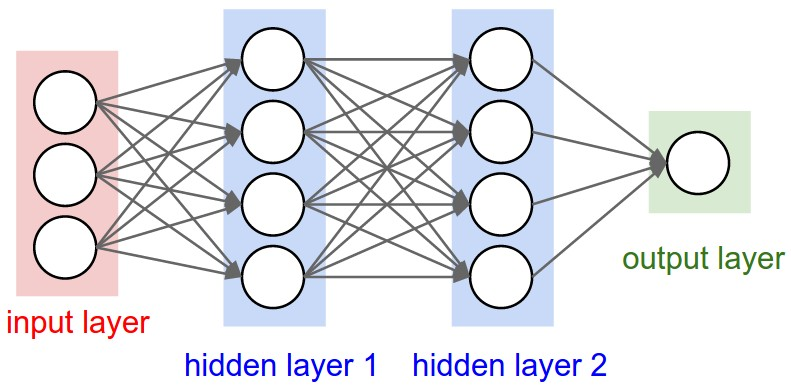
\includegraphics[width = 0.5\hsize]{./figures/neural_net2.jpeg}
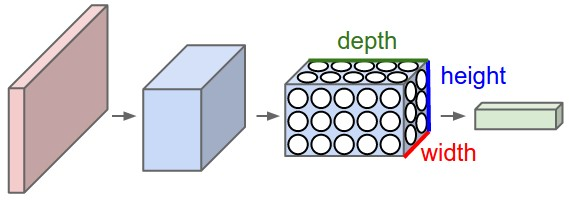
\includegraphics[width = 0.5\hsize]{./figures/cnn.jpeg}
\caption{Regular Neural Network (Left) \cite{StanfordCS231_1} , CNN (right) \cite{StanfordCS231_1}.}
\label{CNNvsNN}
\end{figure}

\subsubsection{Convolutional Layers}
A convolutional layer learns a set of filters, each filter is compact in size, say ($7 \times 7 \times 3$). This filter slides (convolves) over the image, then a dot product is taken between the filter values and the inputs to that filter (Figure \ref{CNN_filter}). The filter slides across with a respective stride, which is a hyperparameter, a stride of one equates to moving one pixel across at a time. A convolutional layer is therefore able to pick up features such as a corner, or higher level features such as the texture of fur. This process creates a 2D activation map containing the response of the filter at each position on the input volume. A number of filters are passed over and a number of activation maps are created, relating to the layer depth which is a tune-able hyperparameter.

\noindent \begin{figure}[h!]
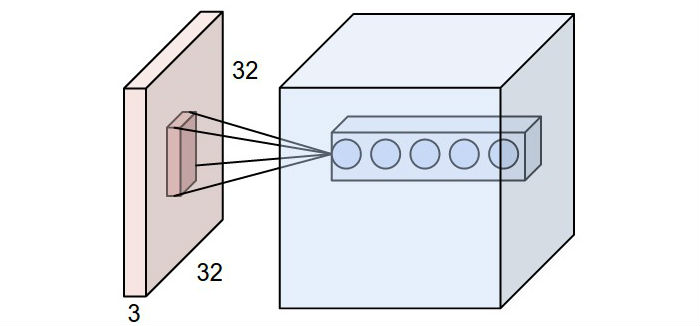
\includegraphics[width = 0.5\hsize]{./figures/conv_filter.jpg}
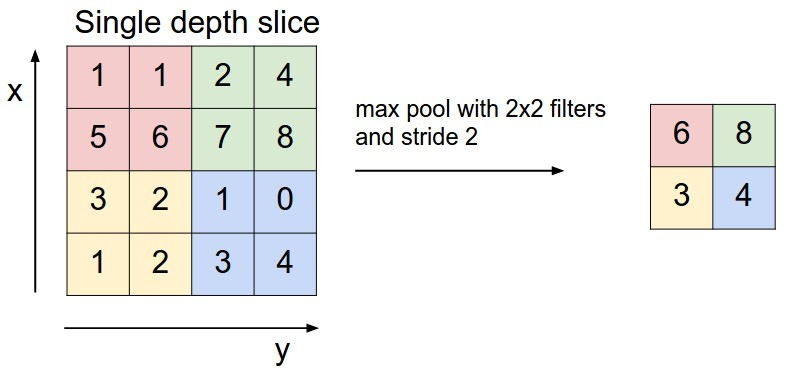
\includegraphics[width = 0.5\hsize]{./figures/maxpool.jpeg}
\caption{CNN Filter (left) \cite{StanfordCS231_conv_filter}, Max Pooling \cite{StanfordCS231_max_pool}}
\label{CNN_filter}
\end{figure}

\subsubsection{Pooling Layers}
Pooling layers are used to reduce the number of parameters in a network. This is a much debated topic, Geoffrey Hinton's paper \cite{DBLP:journals/corr/abs-1710-09829} dicusses the problems of convolutional networks in his 2017 paper and especially focuses on the disadvantages of pooling layers. It is however a current, although fading, method of parameter reduction. For the purposes of optimising network architecture for smaller hardware such as is portable on a bike this is still a recognised and useful method.
\newline \newline
A pooling layer such as that depicted in (Figure \ref{CNN_filter}) passes a kernel over the input (much like in a convolutional layer) and at each spacial location it calculates a metric. For example, max pooling takes the largest value contained within the kernel grid at each consecutive spacial location. This process reduces the input size with respect to the kernel size and the implemented stride.

\subsection{Image Detection} \label{Image_det}
Image detection is an area of research that uses the CNN networks described in Section \ref{Cnn_section}. This is, however, a more difficult task as there can be multiple objects/classes of interest within one image. A naive approach to this problem would be to slide a window across an image and classify at each location. When the network classifies, say a cat at a particular window location it is likely that a cat is located in that area.
\newline \newline
Although the aforementioned approach is valid it would be very slow, not only would it be needed to slide the window over the whole image, the size of the window would also need to be varied. The network cannot know the area of the photo that the object occupies and therefore what size to make the window. There are a number of differing approaches to this problem R-CNN \cite{DBLP:journals/corr/GirshickDDM13} and other later iterations vs YOLO (you only look once) \cite{DBLP:journals/corr/RedmonDGF15}. The R-CNN approach is very similar to the vanilla, naive solution, discussed above (commonly known as exhaustive search) and is used by later techniques for instance segmentation.


\subsubsection{R-CNN} \label{rcnn}
R-CNN, proposed by Ross Girshick et al. \cite{DBLP:journals/corr/GirshickDDM13} in 2014, incorporates a region proposal method. This process produces 2000 proposals which are then passed through a large CNN, and each region is classified using class-specific linear SVMs. This process equates to a 53.7\% mean average precision (mAP) compared to 35.1\% by state-of-the-art methods at the time. In addition to this performance gain the system doesn't rely on far more complicated ensemble methods.
\newline \newline
The region proposal method used is called selective search \cite{Uijlings2013}, this uses a fast segmentation algorithm by Felzenszwalb \cite{Felzenszwalb2004} followed by a greedy algorithm to iteratively group regions together using similarity metrics. The four metrics proposed in the paper are $s_{colour}$, $s_{texture}$, $s_{size}$, $s_{fill}$  the aim is to use a number of metrics to pick up the differences between regions during the growth period and also limit one region's growth at the expense of others (hence the size metric).

\noindent \begin{figure}[h!]
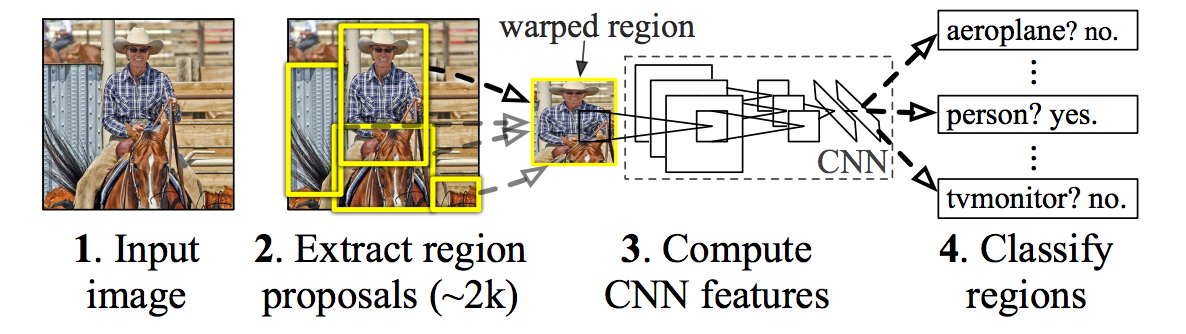
\includegraphics[width = 1.0\hsize]{./figures/region_prop.png}
\caption{R-CNN Region Proposal \& Architecture \cite{DBLP:journals/corr/GirshickDDM13}}
\label{Selective_search}
\end{figure}

The results of the region proposal (Figure \ref{Selective_search}) are a series of windows that are likely to contain an object. These are then simply warped to $227 \times 227$ pixels to fit the input dimension's of the CNN network that follows, containing five convolutional layers and two fully connected layers. The output of the CNN is then fed as a 4096 dimensional feature vector to a set of trained SVMs, one for each class, that are used to score the likelihood for that class. This approach is slow at 13s/image on a GPU and 53s/image on a CPU, the separation of a CNN and SVM is peculiar and adds to this timescale. A later iteration of this method Fast-RCNN is discussed in Section \ref{Fast_RCNN}.

\subsubsection{Fast-RCNN} \label{Fast_RCNN}

R-CNN performs a CNN forward pass for each region proposal and does not share computation between regions \cite{DBLP:journals/corr/Girshick15}. Spacial pyramid pooling networks (SPPnet) \cite{DBLP:journals/corr/HeZR014} are designed to mitigate this problem by creating a feature map (which is always the same shape) from an input image and then classifying each object proposal from a vector extracted from the shared feature map. This paper still uses a multiple-stage classification pipeline but is a marked improvement on R-CNN with regards to speed. 
\newline \newline
Fast-RCNN uses the SPPnet concept but also incorporates a single-stage pipeline. The process inputs an image and multiple RoIs into a fully convolutional network (Figure \ref{Fast_RNN_fig}). Each RoI is then pooled into a fixed-size feature map as in SPPnet and then mapped to a feature vector by fully connected layers. As can be seen in Figure \ref{Fast_RNN_fig} the network then branches into 2 separate outputs, one 4-point regression output of the bounding box location and a K-size classification output, where K is the number of object classes. The model therefore must contain a multi-task loss function that accounts for both bounding box and softmax loss (Equation \ref{multi-task_loss}).

\begin{equation}
\label{multi-task_loss}
L(p,u,t^{u},v) = L_{cls}(p,u) + \lambda[u \geq 1]L_{loc}(t^{u},v)
\end{equation}
in which $L_{cls}(p,u) = -log(p_{u})$ is the log-loss for true class $u$, and $L_{loc}$ is the bounding box regression loss defined as:

\begin{equation}
\label{bbox_loss}
L_{loc} = \sum_{i\in \{x,y,w,h\}}smooth_{L_{1}}(t^{u}_{i}-v_{i}),
\end{equation}
in which

%TODO
\begin{equation}
\label{multi-task_s}
smooth_{L_{1}} = 
\begin{cases}
0.5x^{2} \textnormal{if} x < 1 \\
|x| - 0.5  \textnormal{otherwise} \\
\end{cases}
\end{equation}
is a $L_{1}$ loss. This architecture allows for fast training with the forward pass of the network and therefore processes images 146$\times$ faster than R-CNN due to sharing computation between layers and the improved pipeline design. 

%TODO
\noindent \begin{figure}[h!]
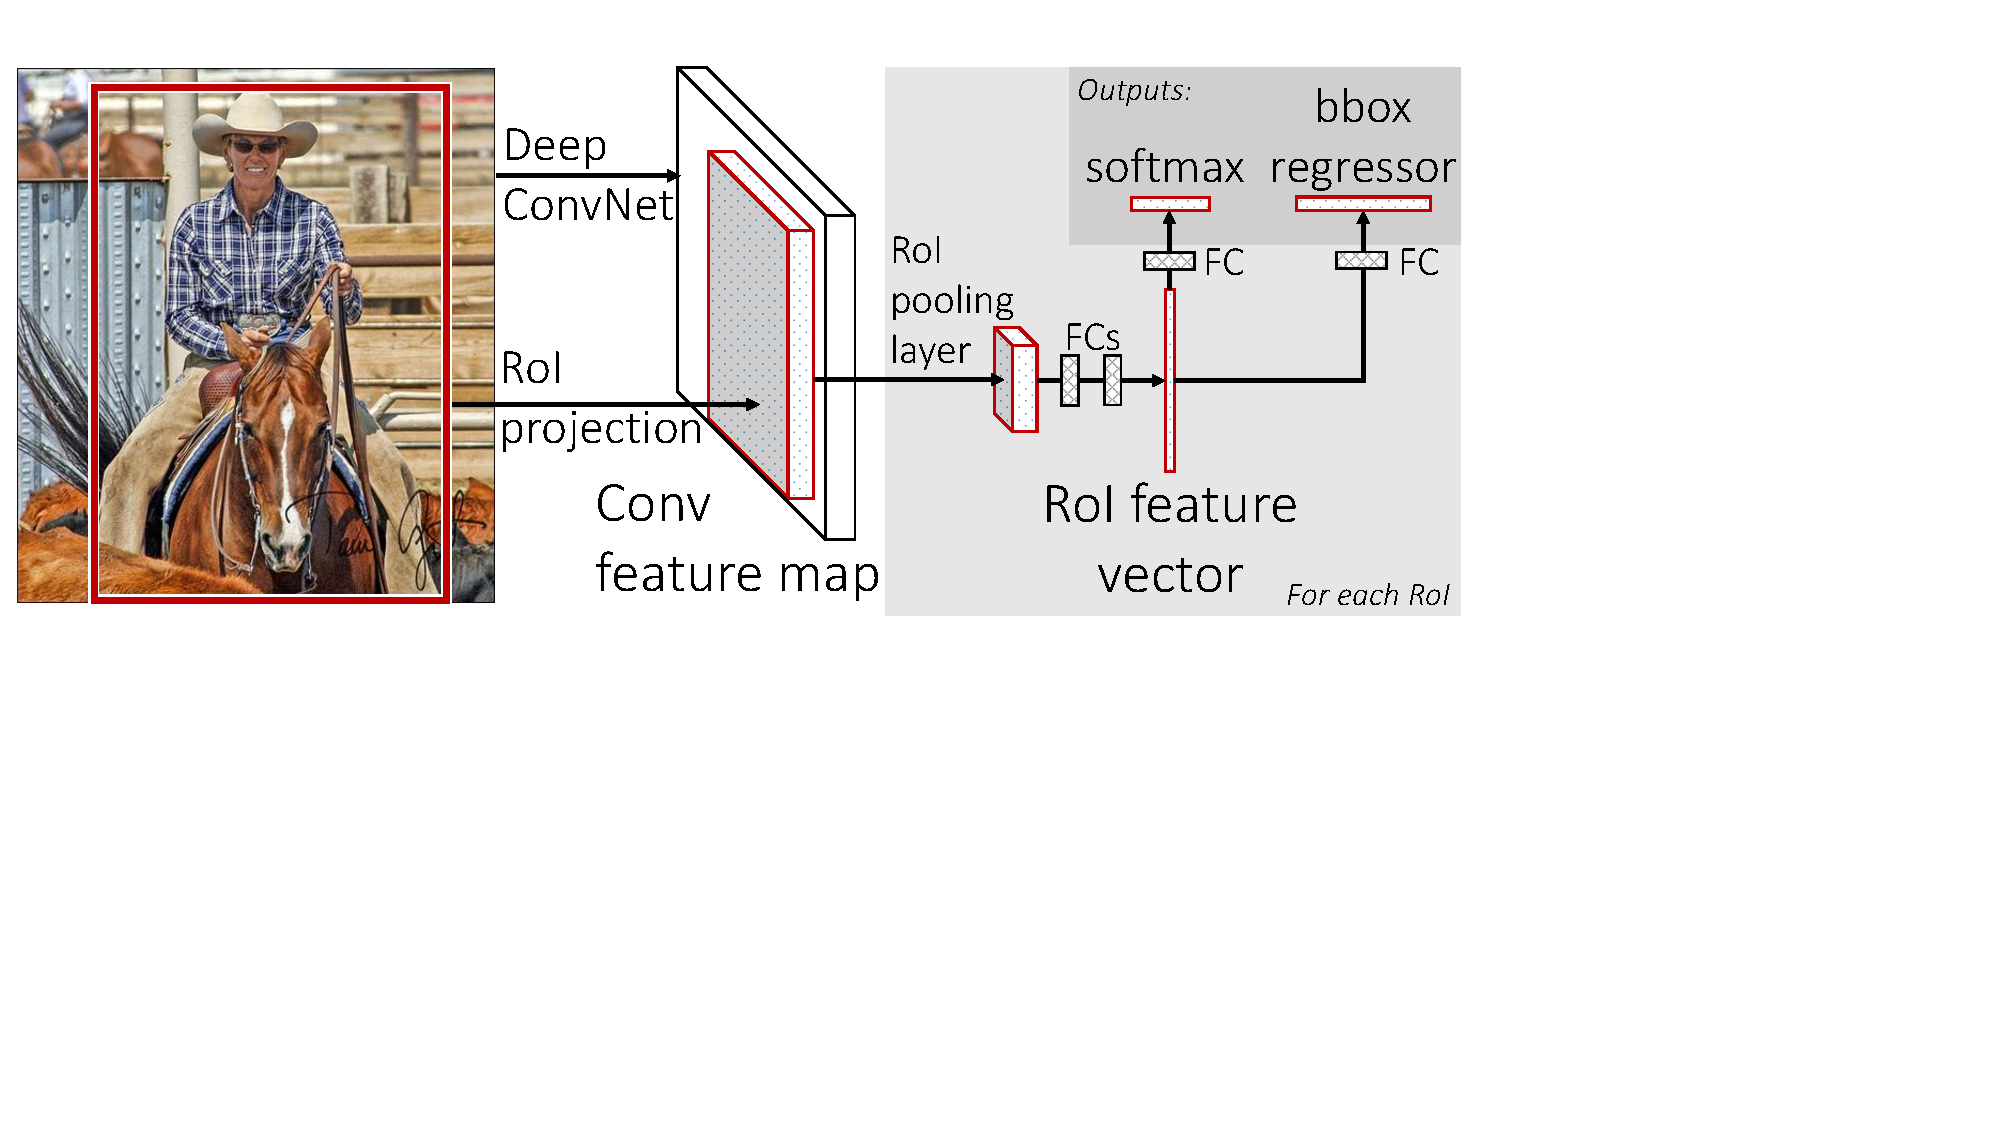
\includegraphics[trim={0 22em 22em 3em},clip,width = 1.0\hsize]{./figures/arch.pdf}
\caption{Fast R-CNN Architecture \cite{DBLP:journals/corr/Girshick15}}
\label{Fast_RNN_fig}
\end{figure}

Figure \ref{Fast_RNN_fig} depicts the network architecture, this incorporates an RoI pooling layer which maps the convolutional feature map from an RoI (created by selective search) to a fixed extent feature map of a set $H \times W$, where $H$ and $W$ are layer hyperparameters. Each RoI is a rectangular window defined by a tuple of four elements ($r,c,h,w$), where ($r,c$) specify the top left corner and ($h,w$) the width. RoI max pooling then divides the RoI window into a grid and then max-pools each grid into the corresponding output cell. The size of the grid is proportionate to the RoI and so the output shape is constant regardless of RoI input size. 

\subsubsection{Faster R-CNN} \label{Faster_rcnn}
Although the previous method \cite{DBLP:journals/corr/Girshick15} removed the need for a multi-stage classification pipeline (CNN and SVM), it still relies on the selective search \cite{Uijlings2013} method for region proposal. This part is now the computational bottleneck that slows down the process. Faster R-CNN proposed by Ren et al. \cite{DBLP:journals/corr/RenHG015} seeks to alleviate this issue by combining region proposal into the CNN. The paper suggests the use of a region proposal network (RPN) to produce the RoIs used later in the network. 

%TODO sort out grphic keep only (c)
\noindent \begin{figure}[h!]
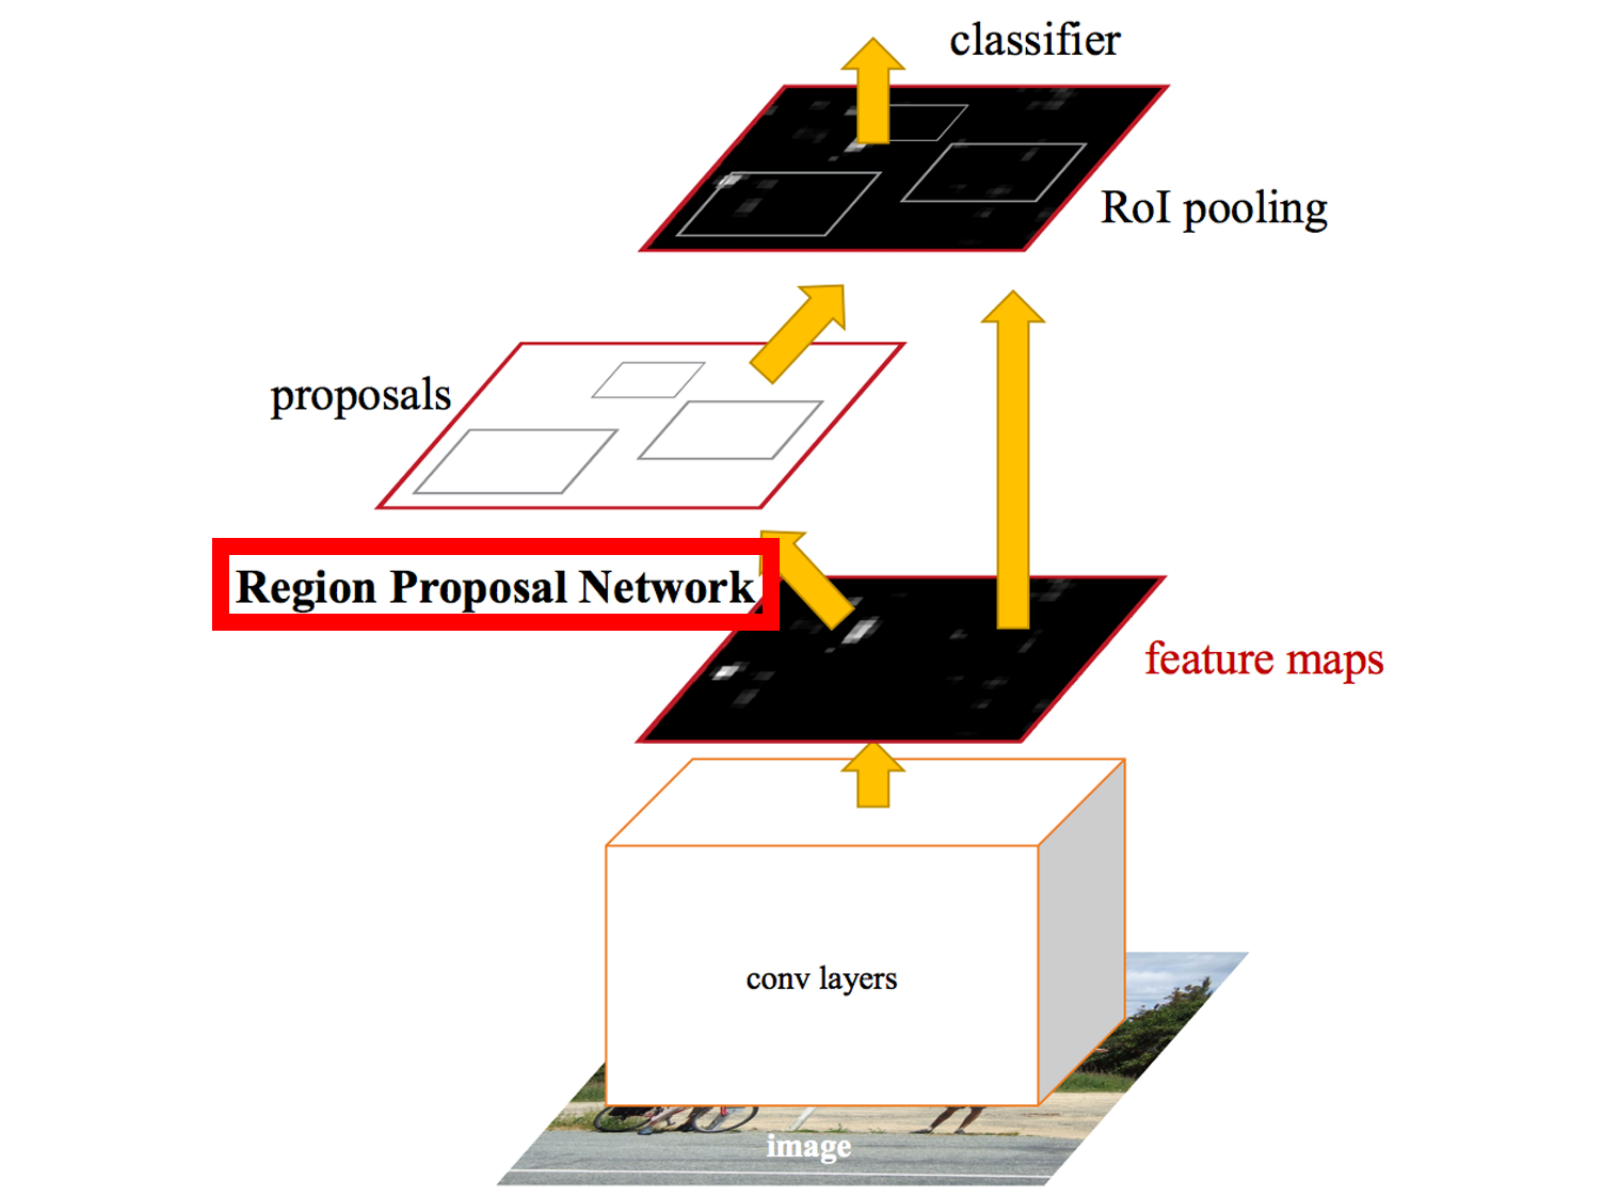
\includegraphics[width = 0.45\hsize]{./figures/faster.png}
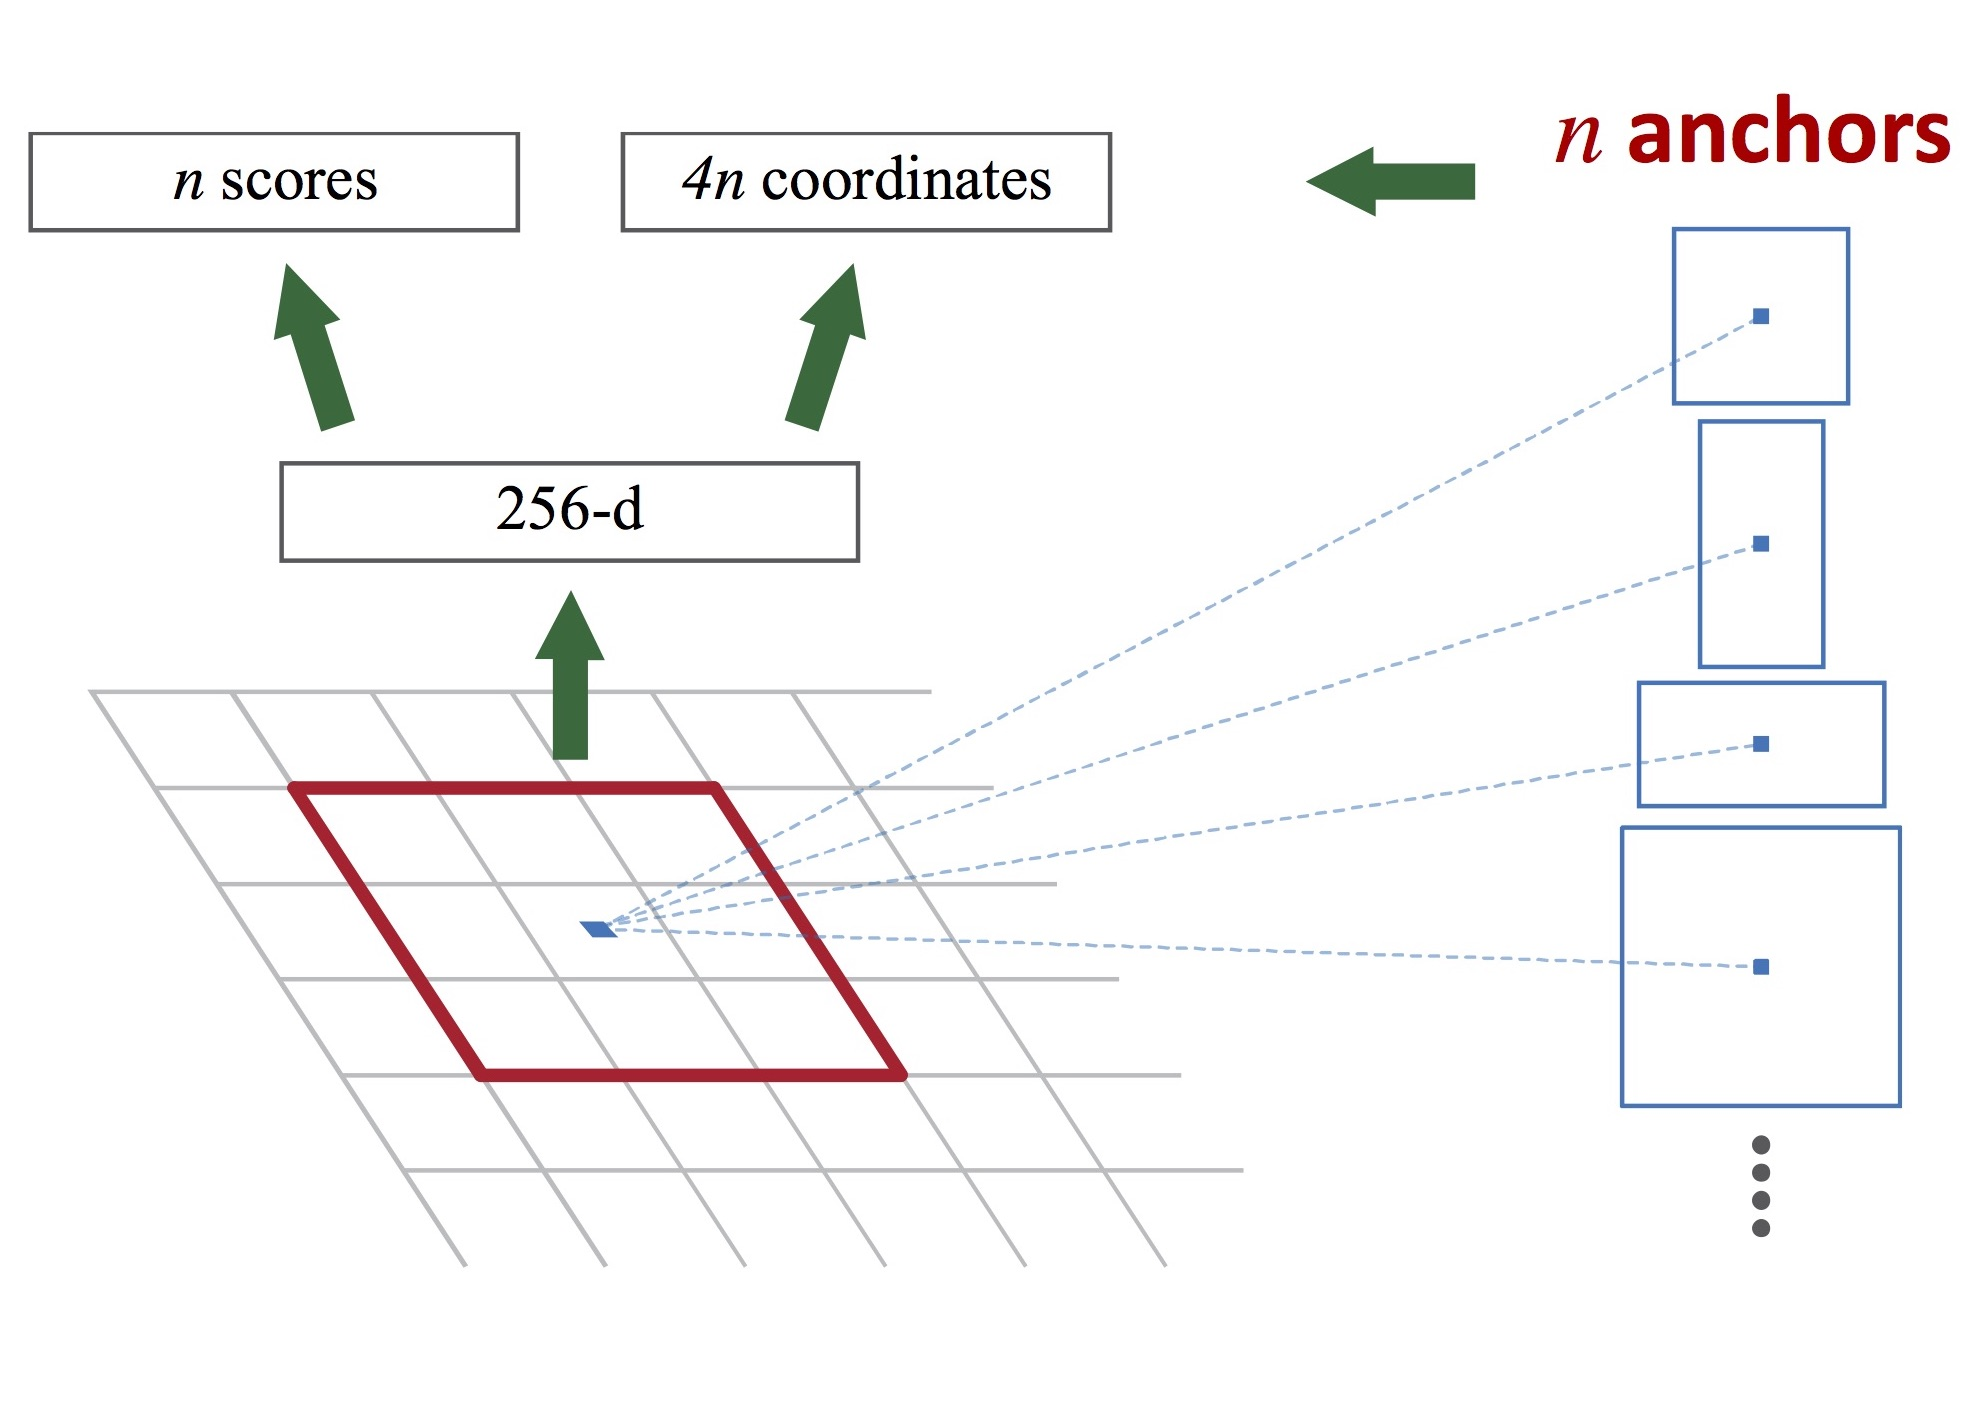
\includegraphics[width = 0.45\hsize]{./figures/rpn_faster.jpg}
\caption{Fast R-CNN Architecture \cite{DBLP:journals/corr/Girshick15}}
\label{Faster_rnn_fig}
\end{figure}

The region proposal network (RPN) outputs a set of rectangular object proposals, each of these proposals has an objectiveness score i.e. how likely the network thinks the proposal contains an object. This part of the network comes after a number of convolutional layers (in this paper 5 or 13 such layers). The region proposals are then created off the feature map from these layers by sliding a smaller network of size $n \times n$ over the convolutional feature map (Figure \ref{Faster_rnn_fig}). At each sliding window location a number of region proposals are predicted simultaneously. These consist of 3 aspect ratios and 3 scales, therefore 9 total region predictions or anchors at each location. The network is then followed by two sibling $1 \times 1$ convolutional layers, one for $reg$ (region proposal) and one for $cls$ (probability of object or not). The $reg$ layer outputs 4$k$ results, which represents the encoding coordinates of the $k$ boxes and the $cls$ later scores the probability that there is an object or no object in each proposal, therefore cls has $2k$ outputs. This results in a convolutional layer output of depth 9.
\newline \newline
The loss for the network is calculated from two metrics, the output of the $reg$ layer is a binary, i.e. positive example, or not. A positive example is defined by how much the box overlaps with the ground truth box of the object and so an IoU (Intersection-over-union) overlap $> 0.7$ is considered a positive example and an IoU $< 0.3$ is considered a negative label. For the first positive case, if no positive examples are found, the boxes with highest IoU  are labelled positive. With this it follows that:

\begin{equation}
\label{multi-task_loss_fast_rcnn}
L(\{p_{i}\},\{t_{i}\}) = \frac{1}{N_{cls}} \sum_{i} L_{cls}(p{i},p_{i}^{*}) + \lambda \frac{1}{N_{reg}} \sum_{i}p_{i}^{*} L_{reg}(t_{i},t_{i}^{*})
\end{equation}

Where $i$ is the anchor index, $p_{i}$ is the predicted probability of anchor $i$ containing an object. The ground truth label $p_{i}$ is denoted as a 1 for a positive anchor and 0 for a negative therefore $L_{reg}$ is only activated for a positive example, $t_{i}$ and $t_{i}^{*}$ represent the 4 coordinates of the bounding boxes, and $L_{cls}$ is the classification loss. The two terms are normalised ($N_{cls}$ and $N_{reg}$) and balanced by a weighting parameter $\lambda$. The final term to discuss, the bounding box regression is calculated, simply, as follows:

\begin{equation}
\begin{aligned}
\label{bounding_box_loss}
t_{x} = (x-x_{a})/w_{a}, \quad t_{y} = (y-y_{a})/h_{a},\\
t_{w} = log(w/w_{a}), \quad t_{h} = log(h/h_{a}), \\
t_{x}^{*} = (x^{*}-x_{a})/w_{a},\quad t_{y}^{*} = (y^{*} - y_{a})/h_{a} \\
t_{w}^{*} = log(w^{*}/w_{a}), \quad t_{h}^{*} = log(h^{*}/h_{a})
\end{aligned}
\end{equation}

where $x$, $y$, $w$, and $h$ are the box centre coordinates plus width and height. Predicted box, and anchored box are denoted by $x$, $x_{a}$, $x^{*}$ (likewise for $y$, $w$, $h$).
\newline \newline
Finally after the regions have been proposed, c.6000 per image, some regions overlap with others, and so, to reduce redundancy non-maximum supression is used on their $cls$ score with an IoU threshold of 0.7 to leave around 2000 proposals per image. Non-maximum supression is a technique that sets all neighbouring areas to zero around a local maximum and hence only keeps the maximum value and suppresses the others.
 
\subsection{Image Segmentation}\label{image_seg}
Unlike the image detection problem described in Section \ref{Image_det}, this task aims to segment an image on a pixel-by-pixel basis into respective classes (Figure \ref{cityscapes_data}). A conventional classification network takes an image and outputs a prediction of which class the image is i.e. a vector of probabilities or a `score'. This process uses fully-connected layers to produce the final output vector which throws away important spacial information used in a segmentation task. Therefore Long et al. \cite{DBLP:journals/corr/LongSD14} propose converting these final layers to convolutional layers, maintaining the spacial information and creating a heatmap output (Figure \ref{cityscapes_data}).

\noindent \begin{figure}[h!]
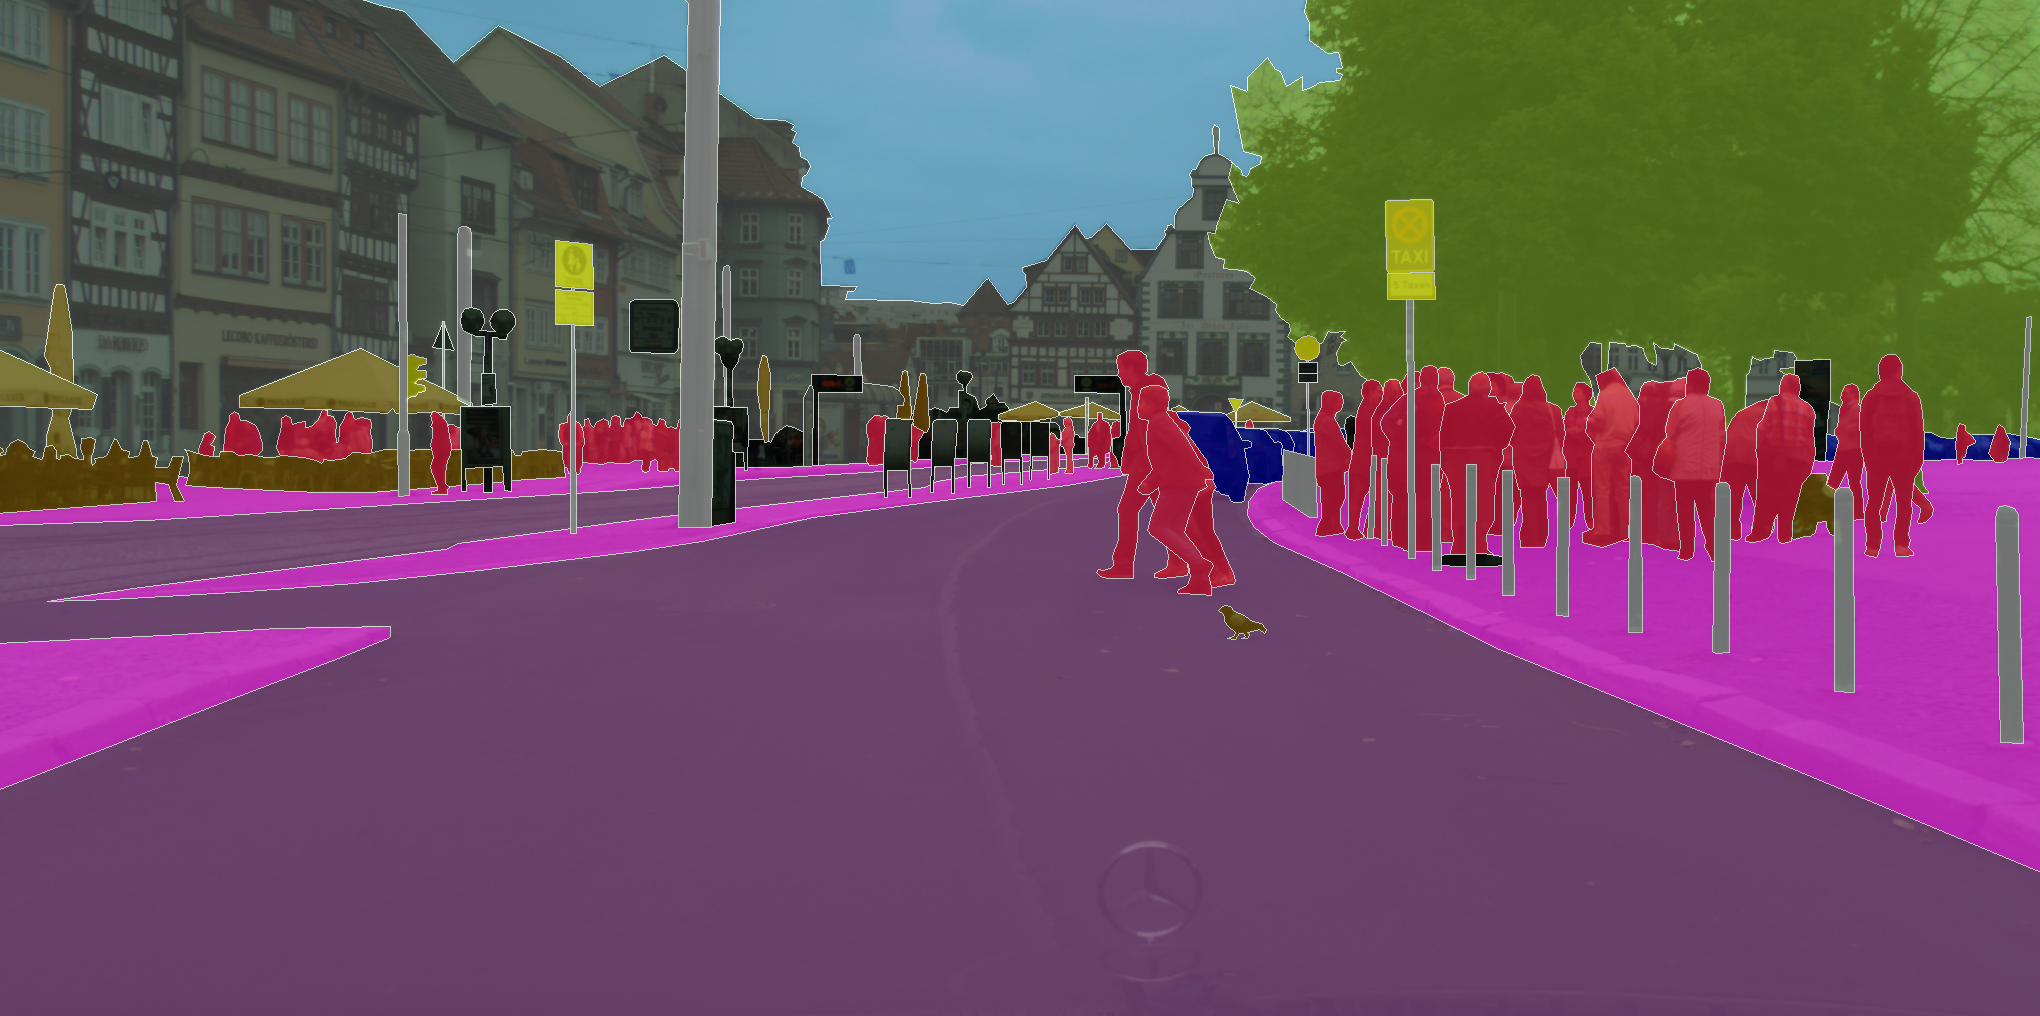
\includegraphics[width = 0.5\hsize]{./figures/image_seg1.png}
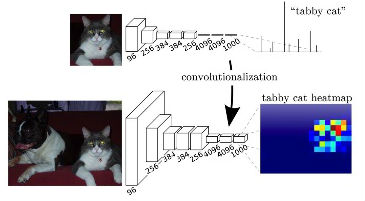
\includegraphics[width = 0.5\hsize]{./figures/sem_im_seg1.jpg}
\caption{Image Segmentation \cite{DBLP:journals/corr/CordtsORREBFRS16}, Convolutional Heat Map \cite{DBLP:journals/corr/LongSD14}}
\label{cityscapes_data}
\end{figure}

The heatmaps produced from the network then need to be upsampled from their respective dimensions to that of the output image. This process is essentially a reverse or deconvolution. Upsampling, therefore, with factor f is convolution with a fractional input stride of 1/f. Essentially each filter is placed on the output image and then multiplied by the input pixel. Hence the image increases in size depending on stride and kernel size as one pixel value is interpolated over a grid. The final problem therefore is how to choose the filter values, this can be done in a number of ways but the main accepted approach is to simply learn them as part of the tuning process.
\newline \newline
An important concept is that of patchwise training which feeds the network a number of patches from an input image (small patches surrounding objects of interest) instead of an entire input image. This both helps to balance the classes, ensures the input has enough variance, and is a correct representation of the input set. However, this paper argues that this can be done from a fully convolutional training regime with incorporating a DropConnect-like mask \cite{Wan:2013:RNN:3042817.3043055} between the output and the loss. A DropConnect mask is similar to the proposed regularisation technique of Dropout \cite{JMLR:v15:srivastava14a} except that it randomly sets the network weights to 0 rather than the activation functions. This, on the output layer (connected to the network loss) is found to have the same effect as patch-wise sampling in Long et al.'s paper.
\newline \newline
Although conventional proven classification architectures performed to state-of-the-art when modified for segmentation (56.0 mean IU), Long at al. \cite{DBLP:journals/corr/LongSD14} go on to design a bespoke network that achieves 62.7 mean IU. Mean pixel intersection over union (Mean IU) is a standard performance metric where the mean is taken over all classes, including the background. The paper describes a network architecture that uses skips \cite{Bishop:2006:PRM:1162264}. Skips allow predictions from lower-level coarser layers to interact with finer, latter layer predictions. This lets the model make local predictions (finer) within the context of the global structure (coarser). This addition made for a marked increase in performance by simply up-sampling earlier layers and summing with latter layer outputs for a final image prediction.

\subsection{Instance Segmentation}
Instance segmentation is a problem that combines research in Sections \ref{Image_det} \& \ref{image_seg}, it aims to not only perform pixel-wise segmentation of classes but also determine instances of objects within and image. As discussed in Section \ref{mask_rcnn} there is a simple method of combining these networks into one simple classification pipeline.
\subsubsection{Mask R-CNN} \label{mask_rcnn}
Mask R-CNN was proposed by Facebook AI Research (FAIR) namely Kaiming He et al. in March 2017. It uses the Faster R-CNN network described in Section \ref{Faster_rcnn} which builds from advances in Sections \ref{rcnn}  \& \ref{Fast_RCNN}. The method works by simply adding a branch from the existing network for predicting segmentation masks as in Section \ref{image_seg} (Figure \ref{Mask_rcnn_arch}). The branch is a small FCN that is applied to each ROI for segmentation. There are a number of slight modifications to each approach to produce the final Mask R-CNN that are documented below.
\newline \newline

\noindent \begin{figure}[h!]
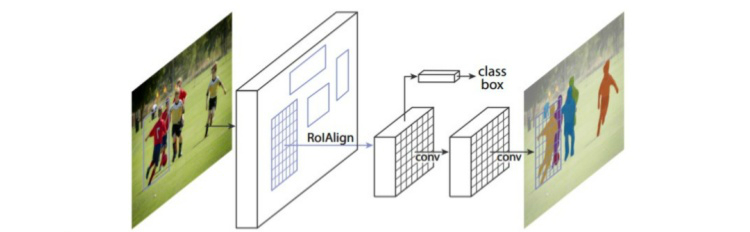
\includegraphics[width = 1.0\hsize]{./figures/mask_arch.jpg}
\caption{Mask R-CNN \cite{DBLP:journals/corr/HeGDG17}}
\label{Mask_rcnn_arch}
\end{figure}
%TODO nice binary mask per class photo
RoIs are produced from the RPN as in Faster R-CNN \cite{DBLP:journals/corr/RenHG015} then an $m \times m$ mask is predicted from each RoI without the use of a fully-connected (fc) layer and therefore keeps spacial information as in Section \ref{image_seg}. It was found during experimentation that it is preferable to decouple the class classification and the mask production of the network. This stops multiple classes disrupting eachother during mask production, hence a mask is produced for each class. The class of each respective mask is then determined from the class output branch and that binary mask is selected. 
\newline \newline
The loss function for the network must now incorporate the three different branches; mask, class prediction, bounding-box prediction (Equation \ref{maskrcnnloss}). 

\begin{equation}
\label{maskrcnnloss}
L = L_{cls} + L_{box} + L_{mask}
\end{equation}

Where $L_{cls}$ \& $L_{box}$ are identical to Section \ref{Fast_RCNN}. The mask branch loss is determined by a per-pixel sigmoid between the ground-truth class ($k$) and the corresponding $k$th binary mask (excluding other classes) and is calculated with an average binary cross-entropy loss.
\newline \newline
RoI pool as discussed in Section \ref{Fast_RCNN} is modified in this approach. Instead of subdividing an RoI into discrete regions e.g. a grid of $4 \times 5$ cells. An RoI does not always divide equally into these grid cells and so rounding of grid sizes is needed, this quantisation of sub-windows can cause misalignments of the RoI and extracted features. The new RoIAlign layer introduced in this paper mitigates this problem by not rounding grid-cells. Mask R-CNN uses bi-linear interpolation (linear interpolation with 2d) to compute the exact values of input features at four regularly samples locations in each RoI window.

\section{Background, SLAM} \label{back_slam}
In order to detect collisions between the bike and obstacles the software must have an understanding of the global environment. The detection described in Section \ref{comp_vis_back} allows mapping, and tracking of dynamic objects in the frame, but distance, path prediction and eventually collision prediction rely strongly on an accurate understanding of 2.5-3D space.

\subsection{Sensors}
The sensors used in this project are an RGBD camera and an IMU. These are both available in the Intel Realsense Camera (ZR300, Figure \ref{realsense_camera}). This camera has a USB cable that both provides the power and sends camera information. An extension cable allows for a laptop to be attached to the camera, from a backpack whilst cycling. Potential problems with this setup are due to juddering of the bike during operation; this could cause tricky footage to analyse and can data loss when the hard-drive is writing to disk. The latter issue can easily be solved by writing to an SSD while cycling.

\noindent \begin{figure}[h!]

\includegraphics[width = 1.0\hsize]{./figures/intel_realsense.jpg}
\caption{Intel Realsense Camera (ZR300)}
\label{realsense_camera}
\end{figure}

\subsection{World and Camera Frame} \label{w_c_frame}

In order to fully understand the bike's location, the environment can be considered from two frames of reference, the world and camera frame. The camera, however, cannot be assumed to produce a perfect image and is hence prone to distortion - some types of camera distortion are shown in (Figure \ref{distortion}).


\noindent \begin{figure}[h!]
	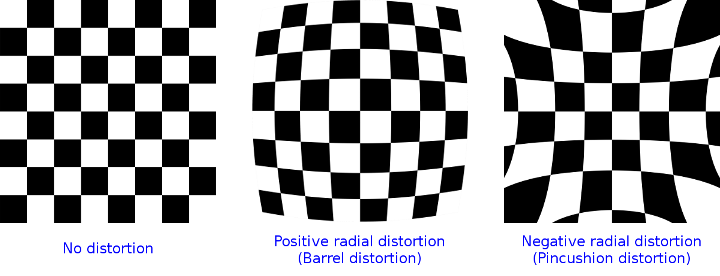
\includegraphics[width = 1\hsize]{figures/distortion_example.png} 
	\caption{No Distortion (left)\cite{opencv_camera_article}, Positive/negative radial distortion (middle/right)}
	\label{distortion}
\end{figure}

A well-known distortion model is "radial-tangential" distortion. As the name implies there is both a radial and tangential component to the distortion (Equation \ref{raddis}) 

\begin{equation}
\begin{aligned}
r^{2} = x_{1}^{'2} + x_{2}^{'2} \\
\mathbf{x''} = \mathbf{d(x')} = \frac{1 + k_{1}r^{2} + k_{2}r^{4}+k_{3}r^{6}}{1+ k_{4}r^{2} + k_{5}r^{4}+k_{6}r^{6}}
\begin{bmatrix}
x'_{1} \\[0.3em]
x'_{2}
\end{bmatrix}
+ 
\begin{bmatrix}
2p_{1}x'_{1}x'_{2} + p_{2}(r^{2} + 2x_{1}^{'2}) \\[0.3em]
p_{1}(r^{2} + 2x_{2}^{'2}) + 2p_{2}x'_{1}x'_{2}
\end{bmatrix}
\end{aligned}
\label{raddis}
\end{equation}

where $x'_{1},x'_{2}$ is the 3d point mapped to the unit plane in z, $k_{1}-k_{6}$ are radial distortion parameters, $p_{1},p_{2}$ are tangential distortion parameters. The model parameters can be determined during camera calibration.

\subsection{Projecting to Camera Frame}

\subsubsection{Calculating the 3D Ray}

\noindent \begin{figure}[h!]
	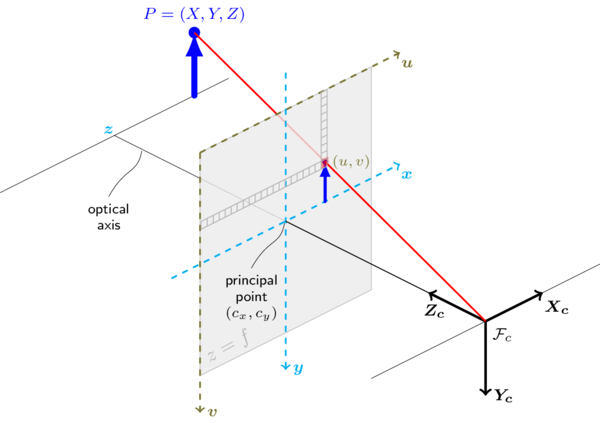
\includegraphics[width = 1.0\hsize]{figures/pinhole_camera_model.png}
	\caption{Pinhole Camera Model}
	\label{pinhole_model}
\end{figure}

Assuming an object or a point on the camera image, it is important to be able to transform such a point into the world frame. To track and gain a 3d appreciation of the environment. Hence for visual context (Figure \ref{pinhole_model}) is a pinhole camera model. The only difference, in practice, in an intermediate un-distorting step to get the point's ray. This is due to the focal lens in the camera, which is not represented in the pinhole model. Hence to find a ray describing a 3d point the image must first be scaled, (Equation \ref{camera_scale})


\begin{equation}
\begin{aligned}
\mathbf{x''} = \mathbf{k^{-1}(u)} = 
\begin{bmatrix}
\frac{1}{f_{1}} & 0 \\[0.3em]
0 & \frac{1}{f_{2}}
\end{bmatrix}
+ 
\bigg (
\mathbf{u} -
\begin{bmatrix}
c_{1} \\[0.3em]
c_{2}
\end{bmatrix}
\bigg )
\end{aligned}
\label{camera_scale}
\end{equation}

where $f_{1},f_{2}$ are x/y focal lengths in pixels, and $c_{1},c_{2}$ is the principal point (image centre) in pixels. The point can be projected to its undistorted location using the reverse of Equation \ref{raddis}.

\begin{equation}
\mathbf{x'} = \mathbf{d^{-1}(x'')}
\label{camera_scale}
\end{equation}

and finally the ray is calculated by remembering that the z component is of length 1.

\begin{equation}
\mathbf{x} = 
\begin{bmatrix}
\mathbf{x'} \\
1
\end{bmatrix}
\label{to_3d_ray}
\end{equation}

\subsubsection{Calculating the 3D Location}

Now that the ray has been determined we have a point on the 3D unit plane of $z=1$. To find the 3D point in the camera frame, a depth measurement, obtained from the depth camera at the same (undistorted pixel location) is required. Hence the final 3D point is:

\begin{equation}
\mathbf{x} = 
\begin{bmatrix}
\mathbf{x'} \\
depth(\mathbf{x'})
\end{bmatrix}
\label{camera_scale}
\end{equation}

Assuming a static camera location, this would be all that is needed to map the space in-front of the camera. However, as the camera moves, the origin, and orientation of the camera frame changes with respect the world frame. Hence the software must not only determine the 3D location of a point in the camera frame but also translate that to a world frame representation.

\subsection{Projecting to World Frame}


\noindent \begin{figure}[h!]
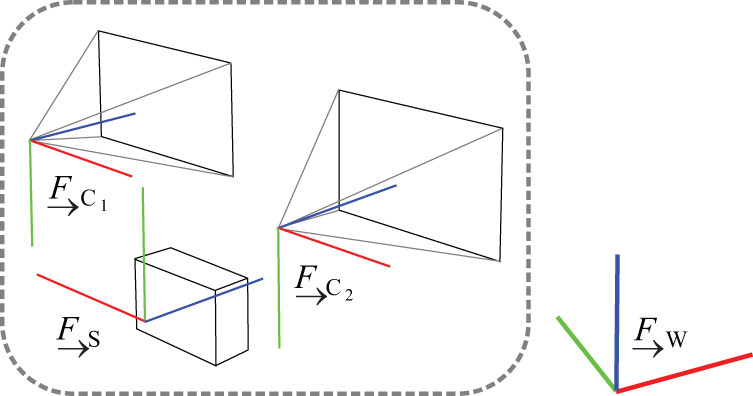
\includegraphics[width = 0.5\hsize]{figures/world_to_cam.jpg}
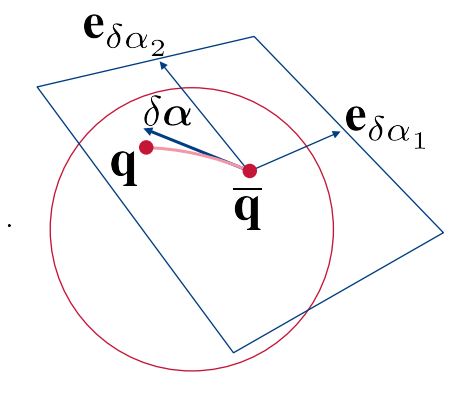
\includegraphics[width = 0.35\hsize]{figures/quaternions.png}
\caption{World vs Camera Frame (left)\cite{Okvis_1}, Hamiltonian Quaternion (right)}
\label{quat_wcs}
\end{figure}


To convert between world (${\xrightarrow{F}}_{W}$), camera frame (${\xrightarrow{F}}_{C_{i}}$), and IMU frame (${\xrightarrow{F}}_{S}$), an appropriate method of describing the orientation, and location of an object in 3D space is needed. A Hamiltonian Quaternion is capable of correctly mapping the orientation of an object in 3D space, it does this by use of a 4D representation of one real part, and 3 imaginary;  

\begin{equation}
\begin{aligned}
\label{quaternion}
q = q_{w} + q_{x}i + q_{y}j+q_{z}k, \\
i^{2}=j^{2}=k^{2}=ijk=-1
\end{aligned}
\end{equation}

With this extra representation of orientation it is possible to map the camera frame to the world frame. Given a position vector in the camera frame $p_{c}$, it can be converted as follows:


\begin{equation}
\begin{aligned}
T_{WC} = T_{WS} \cdot T_{SC} \\
p_{W} = T_{WC} \cdot p_{C} \\
\end{aligned}
\end{equation}

A transformation between frames is represented as $\textbf{T}_{BA}$ where B and A represent reference frames, so $\textbf{T}_{WC}$ converts between the world frame and camera frame. It is composed of a position and orientation transformation:

\begin{equation}
\begin{aligned}
T_{WC} = 
\begin{bmatrix}
C_{WC} & r_{WC} \\
0_{1 \times 3} & 1
\end{bmatrix}
\end{aligned}
\end{equation}

where $T_{WC} \in \mathbb{R}^{4 \times 4}$, the position translation matrix $r_{WC} \in \mathbb{R}^{3 \times 1}$, and the orientation matrix $C_{WC} \in \mathbb{R}^{3 \times 3}$. These transformation matrices must be determined from a SLAM algorithm such as OKVIS which is discussed in the following sections.

\subsection{Bicycle States}

In order to find the bike location and orientation in each frame; a complete representation of the bike's state is needed. At each taken image ($k$) the bike can be assumed to have a set state $\mathcal{X}_{R}^{k}$. Contained within $\mathcal{X}_{R}$ are a set of pose states, $\mathcal{X}_{T}$, and speed/bias states $\mathcal{X}_{sb}$, Equation \ref{states_1}. Landmarks are contained within the set $\mathcal{X}_{L}$.

\begin{equation}
\begin{aligned}
\label{states_1}
\mathcal{X}_{T} := [ _{W}r_{S}^{T},q_{WS}^{T} ]^{T} \\
\mathcal{X}_{sb} := [ _{s}v^{T},b_{g}^{T}, b_{a}^{T} ]^{T} \\
\mathcal{X}_{R} := [ _{W}r_{S}^{T},q_{WS}^{T},_{s}v^{T},b_{g}^{T}, b_{a}^{T}]^{T}
\end{aligned}
\end{equation}

The elements $_{W}\textbf{r}_{S}^{T}$, $\textbf{{q}}_{W}^{T}$ are the position and the quaternion body orientation, $_{s}\textbf{{v}}^{T}$ the velocity, $\textbf{{b}}_{g}$ \& $\textbf{{b}}_{a}$ the accelerometer and gyroscope biases. Since $\delta \textbf{q}$ describes the axis-angle perturbation about the estimate $\overline{q}_{WS}$ it follows that $\textbf{q}_{WS} = \delta \textbf{q} \otimes \overline{q}_{WS}$ """"EXPAND THIS BIT """. Hence the error states combining with (Equation \ref{quat_delta}) are:

\begin{equation}
\begin{aligned}
\label{states_2}
\delta \mathcal{X}_{T} := [ \delta r^{T}, \delta \alpha^{T} ]^{T} \\
\delta \mathcal{X}_{sb} := [ \delta v^{T}, \delta b_{g}^{T},\delta b_{a}^{T} ]^{T} \\
\delta \mathcal{X}_{R} := [ \delta r^{T}, \delta \alpha^{T}, \delta v^{T},b_{g}^{T}, b_{a}^{T}]^{T}
\end{aligned}
\end{equation}


\subsection{The SLAM Problem}

If measurements were exact, mapping of an environment would be easy. This, however is not the case, there is often noise associated with each taken measurement and movement. For example distance measurements and IMU readings are subject both to a noise and a bias (calibration error) which can both be assumed to be Gaussian distributed.

\begin{equation}
\begin{aligned}
\mathbf{\tilde{z}} = \textbf{b}_{c} + s\textbf{M}_{z} + \textbf{b} + \textbf{n} + \textbf{o}
\end{aligned}
\label{measurement_model}
\end{equation}

where $\textbf{z}$ is the correct measurement, $\textbf{b}_{c}$ is a long-term constant bias, $s$ is a scaling factor, $\textbf{M}$ - misalignment, $\textbf{b}$ - time varying bias, $n$ - noise, and $o$ contains other un-modelled influences. This means that no measurement can be trusted exclusively for state-space information. \newline\newline
Historically, before the recent advances in SLAM, it was first assumed that errors have a compounding effect. The position of a bike, would become increasingly unknown as the environment is explored and the bike is displaced from the origin. This makes intuitive sense if say there is only IMU measurements available. At each step, more uncertainty is introduced from the noise and biases (shown in Equation \ref{measurement_model}) and the bike's position becomes more and more uncertain.

For some time it was also presumed to be the case even when external measurements of the environment are taken. This, however, is not the case as proved by Durrant-Whyte \cite{F_Durr_1} since there is a high degree of correlation between estimates of different landmarks and locations in a map, these correlations also increase with successive observations (Figure \ref{slam_prob_fig}). As an example of this (Figure \ref{slam_prob_fig} : Right) displays error in measurements of landmark observation, the mean error is common between all landmarks and so with successive landmark observations, the errors in location estimates become highly correlated. This means that although $\textbf{m}_{i}$'s location may be quite uncertain but the relative location between two landmarks $\textbf{m}_{i}-\textbf{m}_{j}$ is almost certain.\newline\newline 

In the case of the bicycle set-up, there is both an IMU, and a camera. These provide the basic inputs to the OKVIS software \cite{Okvis_1}. Okvis is able to determine the bike's location by optimising the total error, hence combining both the camera and IMU error.

\noindent \begin{figure}[h!]
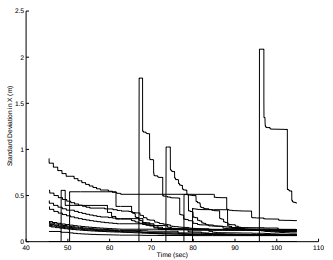
\includegraphics[width = 0.5\hsize]{figures/convergence_landmark_uncertainty.png}
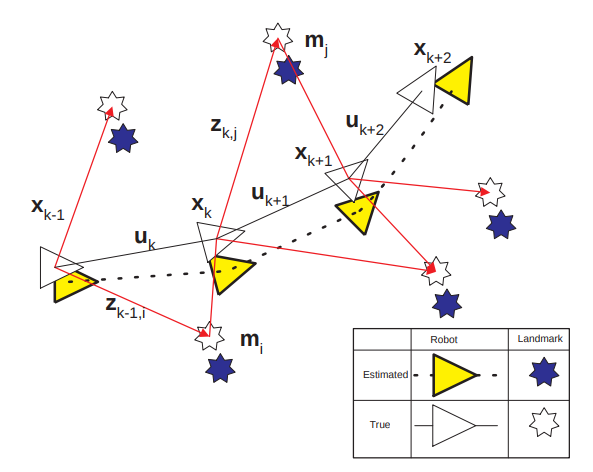
\includegraphics[width = 0.5\hsize]{figures/ess_slam.png}
\caption{Left: Convergence in landmark uncertainty.  Over time, standard deviations reduce monotonically to a lower bound \cite{F_Durr_Pt1}. Right: Error between estimated and true landmarks is common.}
\label{slam_prob_fig}
\end{figure}


\subsubsection{Batch NonLinear Least Squares}

Given an error function for the camera and IMU in the form:

\begin{equation}
\begin{aligned}
J(\mathbf{x}) := \frac{1}{2} \sum_{n=1}^{N} \textbf{e}_{n} (\textbf{x})^{T} \textbf{W}_{n} \textbf{e}_{n}(\textbf{x}) 
\end{aligned}
\end{equation} 

where $\textbf{e}_{n}(\cdot)$ is an error term that is weighted by $\textbf{W}_{n}$, and would consist, in this case of the camera and IMU error. The only way to minimise this error is through observations which are also presumed to have an associated noise term.

\begin{equation}
\begin{aligned}
\textbf{z}_{n} = g_{n}(\textbf{x}) + \textbf{v}_{n},
\end{aligned}
\end{equation} 

where $z_{n}$ is the observation, $g_{n}(\textbf{x})$ the observation model, and $v_{n} ~ \mathcal{N}(0,Q_{n})$ and are independent. Hence as $v_{n}$ is mean 0, the error can be simply formulated by:

\begin{equation}
\begin{aligned}
\textbf{e}_{n}(\textbf{x}) = z_{n} - g_{n}(\textbf{x}), \\
\mathit{error = observation - predicted \textnormal{ } observation}
\end{aligned}
\end{equation}

Since observation noise between the IMU and camera $v_{n}$ are independent the covariance matrix is diagonal. Hence $W_{n} = E[\mathbf{e}_{n} \mathbf{e}_{n}^{T}]^{-1} = Q^{-1}$. The aim of least squares is to find the state vector $mathbf{x}$ that minimises the error function, hence the optimisation problem is posed as:

\begin{equation}
\begin{aligned}
\textbf{x} = argmin(J(\mathbf{x}))
\end{aligned}
\end{equation}

If the error term $\mathbf{e}_{n}(\mathbf{x})$ was linear w.r.t $\mathbf{x}$ the solution would be a simple as setting the $\frac{\delta J(\mathbf{x})^{T}}{\delta \mathbf{x}}$ to zero and solving the respective simultaneous equations. However this is often not the case, and so the solution to the equation must be solved iteratively, with for example, gauss-newton formulation of the equations and a solver such as google-ceres.

\subsubsection{Frame to Frame Matching}



\subsubsection{Camera Re-projection Error}

As discussed in Section \ref{w_c_frame}, the camera uses a lens to take a photograph. This, especially on cheaper cameras, can distort the image. The distortion is intrinsic to the camera and it needs to calibrated to determine a distortion model $\mathbf{d}(^{.})$. This is then used to determine the re-projection error \cite{Furgale}.

\begin{equation}
\begin{aligned}
\textbf{e}_{r}^{i,j,k} = \textbf{z}^{i,j,k} - \textbf{d}_{i} (\textbf{T}^{k}_{CiS} \textnormal{ } \textbf{T}^{k}_{SW} \textnormal{ } _{w}\textbf{l}^{j})
\end{aligned}
\end{equation}

where $\textbf{z}^{i,j,k}$ denotes the measurement image coordinates.

\subsubsection{IMU Kinematics}

Therefore the kinematics of the IMU can be modelled as:

\begin{equation}
\begin{aligned}
\label{imu_kin}
_{W} \textbf{\.{r}}_{S} = \textbf{C}_{WS} \textnormal{ } _{s}\textbf{v}, \\
\textbf{\.{q}}_{WS} = \frac{1}{2} \Omega(\tilde{_{S}\textbf{$\omega$}})\textbf{q}_{WS}, \\
_{S}\textbf{\.{v}}= (_{S}\tilde{\textbf{a}} + \textbf{w}_{a} - \textbf{b}_{a}) + C_{SW} \textnormal{ } _{W}\textbf{g} - (_{S}\textbf{$\omega$}) \times _{S}\textbf{v}, \\
\textbf{\.{b}}_{g} = \textbf{w}_{bg}, \\
\textbf{\.{b}}_{a} = -\frac{1}{\tau}\textbf{b}_{a} + \textbf{w}_{ba}, \\
\end{aligned}
\end{equation}

where:
\begin{equation}
\begin{aligned}
 \Omega(\tilde{_{s}\textbf{$\omega$}}) = \begin{bmatrix}
       -_{S}\textbf{$\omega$}  \\[0.3em]
       0
     \end{bmatrix} ^{\oplus} \\
_{S}\textbf{$\omega$} =  _{S}\tilde{\textbf{$\omega$}} + \textbf{w}_{g} - \textbf{b}_{g}
\end{aligned}
\end{equation}

 $_{W} \textbf{\.{r}}_{S}$ represents the position derivative likewise $_{S}\textbf{\.{v}}$ for velocity,  $_{S}\tilde{\textbf{a}}$ accelerometer measurements, $_{W}\textbf{g}$ earth's gravitational acceleration vector, and finally w:= [$w_{g}^{T},w_{a}^{T},w_{bg}^{T},w_{ba}^{T}$] are independent Gaussian white noise processes with zero mean.
 
 \subsubsection{IMU Kinematics Linearised}
 
 In order to optimise the cost function, it is important to linearise the IMU kinematics. The error dynamics take the form:
 
\begin{equation}
\begin{aligned}
\delta \mathcal{X} \approx  \textbf{F}_{c} (\overline{x}_{R}) \delta \mathcal{X}_{R} + \textbf{G}(\overline{x}_{R})\textbf{w} \\
\end{aligned}
\end{equation}

\begin{equation}
\begin{bmatrix}
       \delta \textbf{\.r}  \\[0.3em]
       \delta \textbf{\.a} \\[0.3em]
       \delta \textbf{\.v} \\[0.3em]
       \delta \textbf{\.b}_{g} \\[0.3em]
       \delta \textbf{\.b}_{a}
\end{bmatrix}
=
\begin{bmatrix}
       0_{3 \times 3} &  [\overline{C}_{WS}\overline{v}]^{\times}
       & \overline{C}_{WS} &  0_{3 \times 3} &  0_{3 \times 3}\\
       
       0_{3 \times 3} & 0_{3 \times 3} 
       & 0_{3 \times 3} &  -\overline{C}_{WS} &  0_{3 \times 3}\\
       
       0_{3 \times 3} & -\overline{C}_{WS}[_{W}\textbf{g}]^{\times}
       & -[_{S}\overline{\omega}]^{\times} &  -[_{S}\overline{v}]^{\times} &  -I_{3}\\
       
       0_{3 \times 3} & 0_{3 \times 3}
       & 0_{3 \times 3} &  0_{3 \times 3} &  0_{3 \times 3}\\
       
       0_{3 \times 3} & 0_{3 \times 3} 
       & 0_{3 \times 3} &  0_{3 \times 3} &  -\frac{1}{\tau}\textbf{I}_{3}
\end{bmatrix}
\begin{bmatrix}
       \delta \textbf{r}  \\[0.3em]
       \delta \textbf{a} \\[0.3em]
       \delta \textbf{v} \\[0.3em]
       \delta \textbf{b}_{g} \\[0.3em]
       \delta \textbf{b}_{a}
\end{bmatrix}
+
\begin{bmatrix}
       0_{3 \times 3}  \\[0.3em]
       \overline{C}_{WS} \textbf{W}_{g} \\[0.3em]
       \overline{C}_{WS} \textbf{W}_{a} \\[0.3em]
       \textbf{W}_{bg} \\[0.3em]
       \textbf{W}_{ba}
\end{bmatrix}
\end{equation}
 
This formulation of the error dynamics is then used to derive the IMU error term (Equation \ref{imu_error_}), for further details see \cite{Okvis_1}.


\begin{equation}
\mathbf{e}^{k}_{s}(\mathbf{x}^{k}_{R},\mathbf{x}^{k+1}_{R},\mathbf{z}_{s}^{k}) = 
\begin{bmatrix}
       _{W} \hat{\mathbf{r}}_{S}^{k+1} - _{W}\mathbf{r}_{S}^{k+1} \\
       
       2[\hat{\mathbf{q}}_{WS}^{k+1} \otimes \mathbf{q}_{WS}^{k+1 \textnormal{ } -1]} \\
       
       \hat{\mathbf{x}}^{k+1}_{sb} - \mathbf{x}_{sb}^{k+1}
\end{bmatrix}
\label{imu_error_}
\end{equation}



\subsubsection{Keypoint Detection}\label{BRISK_section}

The Okvis \cite{Okvis_1} paper uses an corner detection method to determine keypoints and then matches these keypoints using a binary descriptor (BRISK \cite{BRISK}). Binary descriptors use a sampling pattern to create pairs of points (lines). The algorithm then compares the two points ($p1,p2$) and if $p1 > p2$ a 1 is recorded and otherwise 0. This creates a binary string, that along with orientation representation describe a keypoint. When matching keypoints between images a simple, and fast $\sum XOR(img1,img2)$ reveals keypoint similarity from which a threshold can be used to determine matches.

\noindent \begin{figure}[h!] 
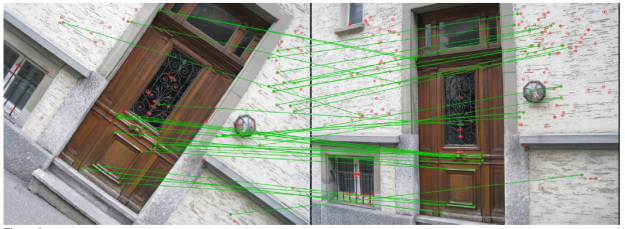
\includegraphics[width = 0.7\hsize]{figures/brisk.jpg}
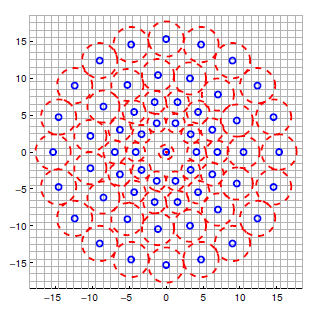
\includegraphics[width = 0.26\hsize]{figures/brisk.png}
\caption{Left: Brisk keypoint matching example, Right: Brisk Sampling Pattern \cite{BRISK} }
\label{Brisk}
\end{figure}

The BRISK sampling pattern (Figure \ref{Brisk}: Right) uses a standard Gaussian smoothing at each sample point. The standard deviation of the sample is represented by the red circles in the figure. This ensures the sample is less prone to noise than other traditional binary detectors e.g. BRIEF.


\section{Background, Object Tracking}

Once an object is found (Section \ref{comp_vis_back}) and the 3d world coordinates of the object in question (bike, car, pedestrian etc.) are determined (Section \ref{back_slam}) the path of the object needs to be calculated. This requires the ability to track an object from frame-to-frame and transfer that knowledge to 3D space. Mask-RCNN as an instance segmentation solution (Section \ref{comp_vis_back}) and runs slower than real-time unless on a powerful GPU system, which cannot be feasibly carried on a bike. So once an object is detected it is preferable to learn simpler features and track it with more basic but faster techniques. An object from frame-to-frame can be easily distinguished if the features of that object are not occluded and colour balance (for example sunny to shaded regions) is minimal. This, however, is not the case in real-world environments and so the tracking task is less simple than it appears.
\newline \newline
Section \ref{back_slam} used the IMU measurements and camera measurements to determine the location of the bicycle and objects in the world frame. This problem is similar but involves the tracking of an object. In \cite{Ped_tract} there are two parts at play, the camera measurements, and a predictive Kalman filter using the object's motion information. The Kalman filter creates a bounding box of the expected object location, the object is then correctly located in that region, and the Kalman filter is then updated.



\subsection{CamShift}

Camshift is a modification of the Meanshift algorithm that locates the maximum of a density function. In this case the probability of a region containing the colour and hue values of a previously discovered object in a new frame. It is an iterative algorithm that starts with an initial estimate $\mathbf{x}$ and a Kernel function $\mathbf{K}(\mathbf{x_{i}} - \mathbf{x})$ which determines the weighting of nearby points for mean re-estimation.

\begin{equation}
m(x) = \frac{\sum_{x_{i} \in N(x)} K(x_{i} - x) x_{i}}{\sum_{x_{i} \in N(x)} K(x_{i} - x)}
\end{equation}

Where N(x) is where $K(x_{i} \neq 0)$. This, however does not account for objects moving in a frame and therefore a dynamic scaling approach is needed where the kernel size is variable. Hence CamShift \cite{Bradski98computervision} solves these issues by updating the window size every time mean shift converges until a required threshold is reached.
\newline \newline
The Meanshift and Camshift algorithms require a probability density to describe objects in each image. Since, as mentioned earlier, colour values in the RGB space can easily alter due to occlusion and other light-variation effects it is suggested in \cite{Ped_tract} to convert the image to an HSV space before creation of a 48-bin histogram. HSV uses hue, saturation and brightness and the transformation from RGB is as follows:

\begin{equation}
\begin{aligned}
H = 
\begin{cases}
    60 \times \Big[ \frac{g-b}{max(r,g,b)-min(r,g,b)} \Big] , if(r = max(r,g,b)) \\
    60 \times \Big[ \frac{b-r}{max(r,g,b)-min(r,g,b)} + 2 \Big] , if(g = max(r,g,b)) \\
    60 \times \Big[ \frac{r-g}{max(r,g,b)-min(r,g,b)} + 4 \Big] , if(b = max(r,g,b))
\end{cases} \\
S = \frac{max(r,g,b)-min(r,g,b)}{max(r,g,b)} \\
V = max(r,g,b)
\end{aligned}
\end{equation}

where H, S and V are the hue, saturation, and brightness value of each pixel and r,g,b are red, green and blue values.

\subsection{Object Tracking Summary}

The method discussed in this section uses image segmentation, a predictive Kalman filter with movement information, and the Camshift algorithm. The update step of the Kalman filter requires a measurement, this is obtained from the Camshift algorithm that iteratively and accurately locates the mid-point of a object in the image. This then updates the Kalman filter which predicts where the object will be in the next image and hence dictates where Camshift starts from at step $k+1$. This means that the expensive Mask-RCNN needs to be called far less frequently and hence makes the entire system less computationally expensive. The architecture used in \cite{Ped_tract} is displayed below (but uses a different image segmentation method of SVMs and Adaboost) in Figure \ref{Ped_tr_mod_fig}.

\noindent \begin{figure}[h!]
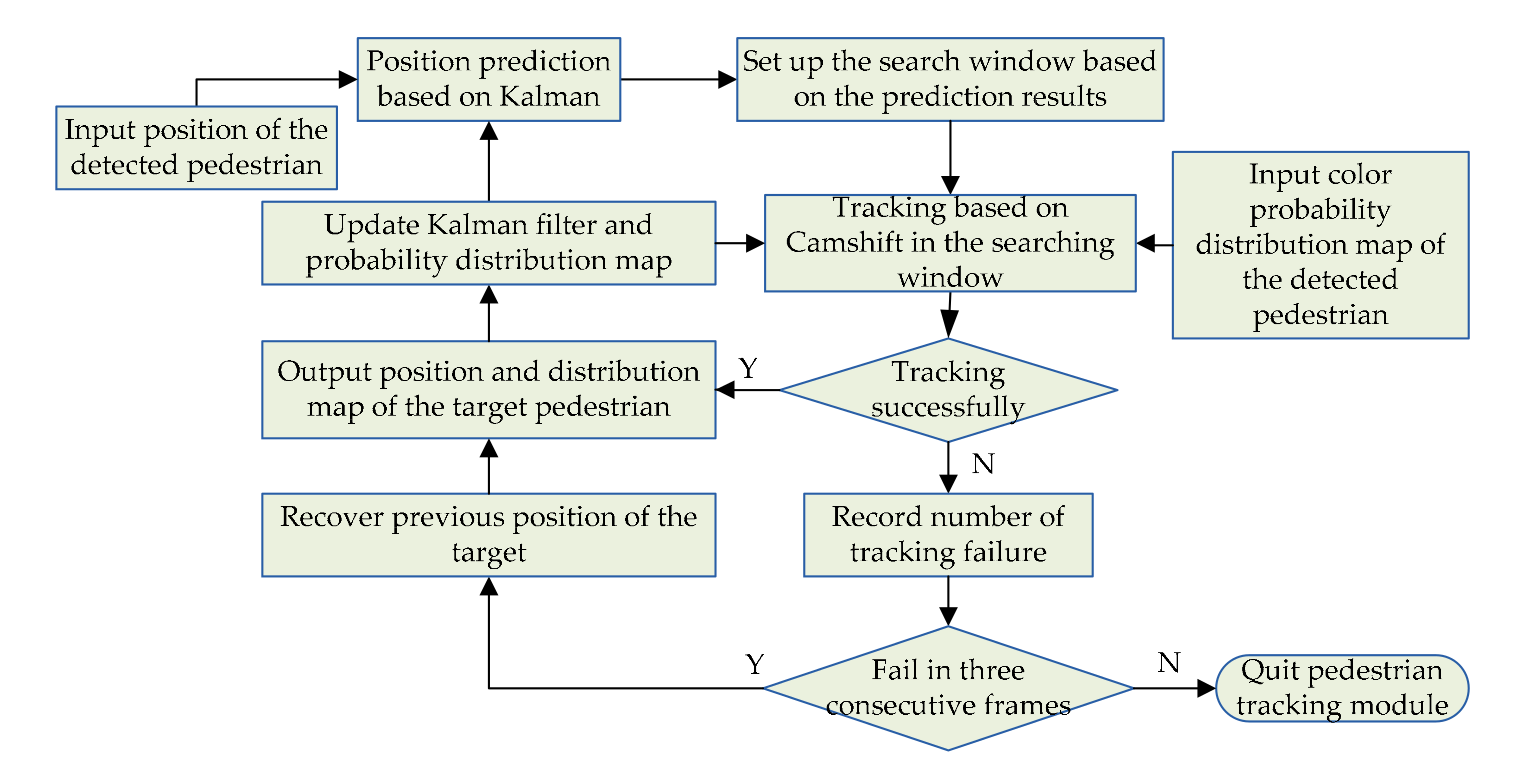
\includegraphics[width = 1.0\hsize]{figures/pedestrian_tracking_module.png}
\caption{Pedestrian Tracking Module \cite{Ped_tract} }
\label{Ped_tr_mod_fig}
\end{figure}

\newpage

\section{Ethics}

\subsection{Modification for Military Purposes}
The code presented in this report, although strictly for civilian applications does have the potential to be modified for military use. It obviously provides the ability to track people and objects from frame-to-frame. This however, is not in a real-time context at present and would require significant modification for use in such an environment that would be conducive to a military application. However, that being said little modification is needed for a simple tracking application from CCTV data for example. This would not need to run at real time and could be a potential source of misuse.

\subsection{Other Ethics Issues}

The code developed is intended to offer a basis for an early warning system to cyclists in urban environments. Hence a number of the inherent ethical problems with, for example the autonomous vehicle space are also applicable to this project. The potential over-reliance on such a system of cyclists could be dangerous and allow for lack of attention and potential accidents when the system is unable to detect a collision. That having been said, it is evident that there is a need for such a system for cyclists and so the benefits would clearly outweighs the disadvantages in such a case.

\section{ROS}

The program is split into respective parts, camera driver, okvis, Mask RCNN and a tracking component. These are all required to communicate for a comprehensive system, hence, since the Mask RCNN implementation used is written in python and okvis plus the driver in c++ ROS is an easy method to transfer messages between nodes. ROS uses a subscriber and publisher methodology where a node can subscribe or publish to a topic. ROS is the de-facto standard library for robotics and allows cross-language compatibility between python and c++.
\newline \newline
The ROS library is optimised for development of robotics applications with useful graphing, message passing and debugging capabilities. In particular ROS supports a rosbag capability which allows the recording and playback of data. This should allow for easy testing of the application in less-than real-time as Mask RCNN operates at 0.2s/frame on a dedicated GPU.


\section{Frame-to-Frame Tracking}

For each frame Mask RCNN outputs a set of bounding boxes, and masks. These are not within any particular order and so a method must be devised to track objects from one frame to the next. This is a hard challenge due to object occlusion, variation in shadow/lighting conditions and rapid in-frame movement. An obvious method is intersection over union (IOU) of the bounding boxes on a frame-by-frame basis. This is good in theory, however, it lacks the ability to compensate for rapid movement (of the object and the camera angle), occlusion and object overlapping. A set of methods have therefore been developed to overcome this problem, which combined provide a robust tracking system.

The method must both track objects in the frame, determine which objects are no-longer in-frame and find any new objects that enter the frame. Information about each object must be stored as to determine the velocity and direction of travel/ if a collision is likely between the cyclist and the object in question. Figure \ref{roi_match} displays an example of a working system.

\noindent \begin{figure}[h!]
	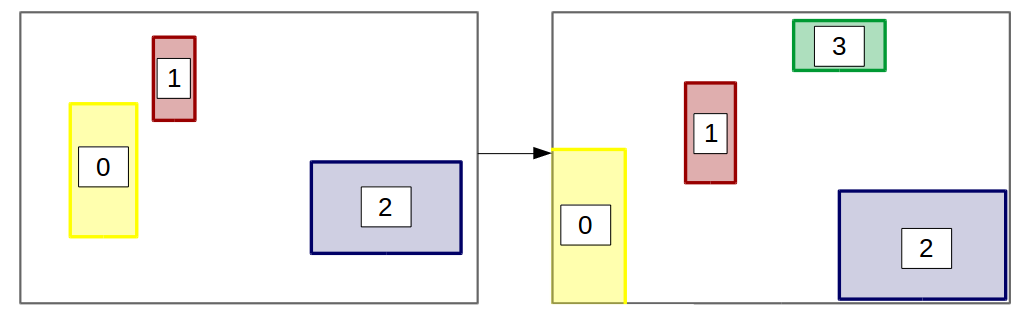
\includegraphics[width = 1.0\hsize]{figures/roi_match.png}
	\caption{ROI Old to New Frame Example.}
	\label{roi_match}
\end{figure}


\subsection{Kernelised Correlation Filter}

Object tracking has been recently advanced by means of discriminative learning methods, these methods try to distinguish between the object and the environment that it is in. The model must therefore be fed negative samples to understand the relevant environment. In the recent paper by Henriques et al. \cite{kcf} the tools are developed to supply thousands of negative samples without iterating over them explicitly. The paper makes use of circulant matrices to provide negative samples. These are obtained by translating the data using a \textit{cyclic shift operator}, which in the 1D signal case is:

\begin{equation}
P = 
\begin{bmatrix}
0 & 0 & \dots & 0 & 1 \\
1 & 0 & \dots & 0 & 0 \\
0 & 1 & \dots & 0 & 0 \\
\vdots & \vdots & \vdots & \ddots & \vdots \\
0 & 0 & \dots & 1 & 0
\end{bmatrix}
\end{equation} 

Therefore the product of $P\mathbf{x} = [x_{n},x_{1},x_{2},...,x_{n-1}]$ and any shift can be modelled using $P^{u}\mathbf{x}$. Because of its cyclic nature, the signal $\mathbf{x}$ repeats when $u=n$ and so the full set of shifted signals is obtained with ${P^{u}\mathbf{x} | u=0,...,n-1}$. An example of this is shown in the 1D case by Figure \ref{circular_data}.

\noindent \begin{figure}[h!]
	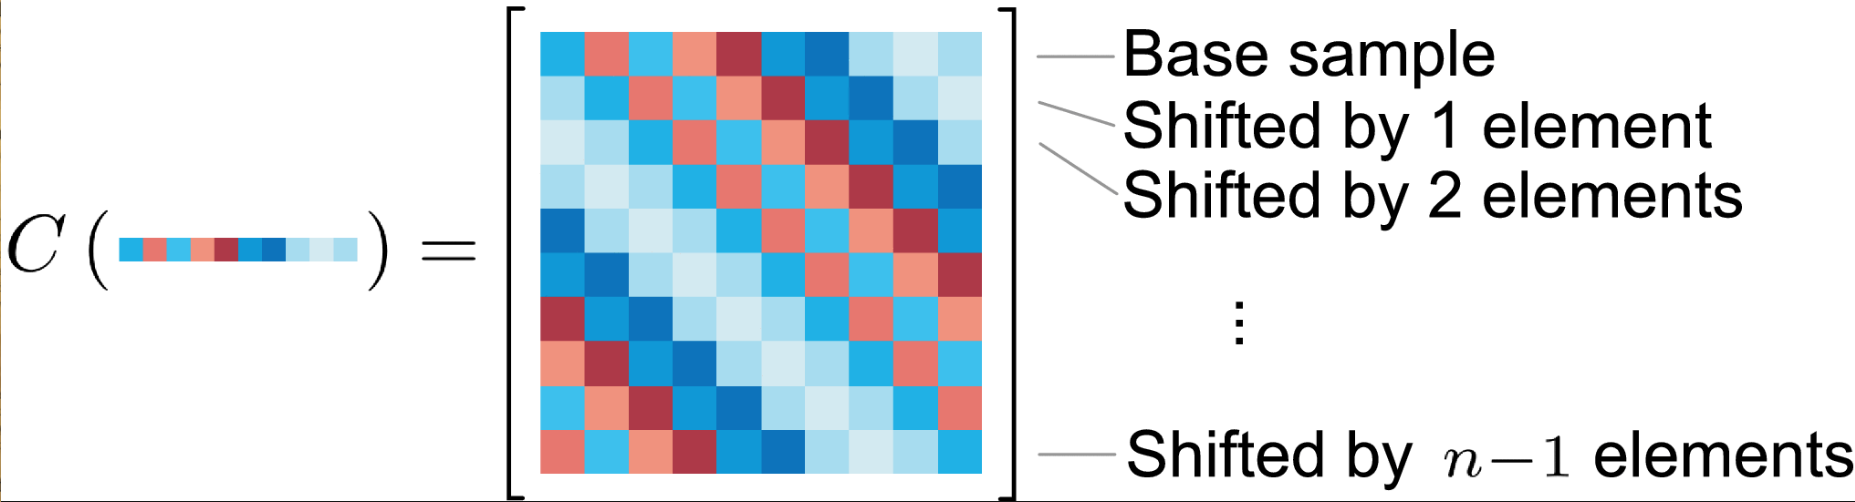
\includegraphics[width = 1.0\hsize]{figures/circular_shift.png}
	\caption{Illustration of circulant matrix.\cite{kcf}}
	\label{circular_data}
\end{figure}

Therefore to compute the regression with shifted samples, the data matrix $X$ takes the form:

\begin{equation}
X = C(\mathbf{x}) = 
\begin{bmatrix}
x_{1} & x_{2} & \dots & x_{n-1} & x_{n} \\
x_{n} & x_{1} & \dots & x_{n-2}  & x_{n-1}  \\
x_{n-1} & x_{n} & \dots & x_{n-3} & x_{n-2}  \\
\vdots & \vdots & \vdots & \ddots & \vdots \\
x_{2}  & x_{3}  & \dots & x_{n} & x_{1} \\
\end{bmatrix}
\end{equation}

Noting that all circulant matrices can be diagonalised by the Discrete Fourier Transform (DFT) $X$ can be written as:


\begin{equation}
\begin{aligned}
\mathit{F}(\mathbf{z}) = \sqrt{n}F\mathbf{z} \\
\hat{\mathbf{x}} = \mathit{F}(\mathbf{x}) \\
X = F diag(\hat{\mathbf{x}}) F^{H}
\end{aligned}
\end{equation}

This is possible because the DFT is a linear operation. 

\subsubsection{Kernels}

Using a kernel, the model can implicitly use a high-dimensional feature space. The kernel function used to do this (e.g. Gaussian), Equation \ref{gauss_kernel} creates an $n \times n$ kernel matrix $K_{i,j} = k(\mathbf{x}_{i},\mathbf{x}_{j})$

\begin{equation}
k(\mathbf{x},\mathbf{x}') = exp (\frac{1}{\sigma^{2}} ||\mathbf{x} - \mathbf{x}'||^{2})
\label{gauss_kernel}
\end{equation}

and therefore the function becomes:

\begin{equation}
f(\mathbf{z}) = \mathbf{w}^{T}\mathbf{z} = \sum_{i=1}^{n} \alpha_{i}k(\mathbf{z},\mathbf{x}_{i})
\end{equation}

with the solution of kernelised Ridge Regression given by:

\begin{equation}
\mathbf{\alpha} = (K + \lambda I)^{-1} \mathbf{y}
\label{kernel_soln}
\end{equation}

where $K$ is the kernel matrix and $\mathbf{\alpha}$ is the vector of coefficients $\alpha_{i}$. Given a kernel function that combines data through a commutative operation, it can be proven that given circulant data the kernel matrix $K$ is also circulant and therefore the DFT trick can be used. This leads to a diagonalisation of Equation \ref{kernel_soln} to Equation \ref{al_soln}.

\begin{equation}
\mathbf{\hat{\alpha}} = \frac{\mathbf{\hat{y}}}{\mathbf{\hat{k}}^{\mathbf{xx}} + \lambda}
\label{al_soln}
\end{equation}

where $\mathbf{\hat{k}}^{\mathbf{xx}}$ is the first row of the kernel matrix $K = C(\mathbf{\hat{k}}^{\mathbf{xx}})$, and a $\hat{ }$ denotes the DFT of a vector. This means that only an $n \times 1$ kernel matrix needs to be computed, due to the circulant kernel property and DFT. This makes the method far faster than conventional kernel methods that require an $n \times n$ sized kernel matrix. Since the bbox prediction is so fast for the KCF tracker; it can be used in conjunction with the other tracking methods mentioned in Sections \ref{BRISK_matching}, \ref{class_matching}, and \ref{kalman_matching}.
\newline
\newline
The kcf tracking algorithm outputs a bounding box which is the predicted coordinates of the object in the next frame. This can be compared to Mask-RCNNs output through a simple matching process. A box in the new frame predicted by Mask RCNN $[x_{mask},y_{mask},width_{mask},height_{mask}]$ can be scored by sampling the pdf from a multivariate Gaussian, in 4D, with mean $[x_{kcf},y_{kcf},width_{kcf},height_{kcf}]$ and covariance matrix $20 \times I_{4 \times 4}$ which translates to a $\sigma^{2} = 20$ for $x,y,width,height$ respectively. This score can then be used in Section \ref{matching_combining_methods} to be combined with the other tracking modules.


\subsection{BRISK - Selector} \label{BRISK_matching}
BRISK as described earlier in Section-\ref{BRISK_section} is a binary descriptor that can match keypoints across two photographs. This can be used also in the tracking section to match keypoints across ROIs, although not thoroughly accurate, it offers a method of matching ROIs regardless of location. This should help re-detect objects after periods of occlusion or overlapping with others that IOU would be unable to do. The process is simple to match the ROIs. First keypoints and descriptors are calculated for each ROI, these are then compared using the fast binary matching process of BRISK, then the Hamiltonian distance is calculated for each matching keypoint...



\subsection{Class Matching} \label{class_matching}
An obvious additional requirement is the matching of classes between frames, as a person's ROI should not match to the ROI of a car in the next frame. Hence for each ROI, the class is stored for access by the next frame. This can both reduce expensive computation time of other metrics but provides an easy ROI comparison tool. It can be noted though that Mask RCNN is not perfect and often mis-classifies objects. It is, however, reliable enough to be assumed as correct.

\subsection{Kalman Filter ROI Matching} \label{kalman_matching}

The Kalman filter has two main parts, a predictive step and an update. The predictive step tries to find a-priori estimates of the state for the next time-step by projecting forward the current state and error covariance estimates. This estimate is then updated using the measurements (camera) of the object location. The iterative process continues improving the Kalman filter estimates at each stage.

\subsubsection{Kalman Predictive Step}
Assuming a linear system with Gaussian process, the state can be modelled as:

\begin{equation}
\begin{aligned}
\hat{X}_{k} =  F_{k} \hat{X}_{k-1} + w_{k-1}
\end{aligned}
\end{equation}

where $k$ is the time step, $\hat{X}_{k} \in \mathbb{R}^{n}$ is the state vector, $F_{k}$ is the $n \times n$ state transition matrix from state $k$ to $k+1$ and $w_{k}$ is $\mathcal{N}(0,Q)$. The state vector is described as follows:

\begin{equation}
\begin{aligned}
\hat{X}_{k} =  [Cx,Cy,w,h,Cx_{vel},Cy_{vel},w_{vel},h_{vel}]
\end{aligned}
\end{equation}

where $(Cx,Cy)$ is the centre point of the bounding box of the object, $w$ the width and $h$ the height. $Cx_{vel}$ describes the centre point velocity in the x direction, and $Cy_{vel},w_{vel},h_{vel}$ the y direction, w the width and h the height. $[Cx,Cy,w,h]$ describe the measurable variables of the system, and there are no controllable parameters in this system. From basic equations of motion, a general measurable parameter $\gamma$, and corresponding velocity  $\gamma_{vel}$ follows the update rule:

\begin{equation}
\begin{aligned}
\gamma_{k+1} = \gamma_{k} + \gamma_{vel} \times \Delta t \\
\gamma_{vel,k+1} = \quad \gamma_{vel,k}
\end{aligned}
\end{equation}

where $\Delta t$ is the time step between each frame. Therefore, the update matrix for the filter $F_{k} \in R^{8 \times 8}$ is as follows:

\begin{equation}
F_{k} = 
\begin{bmatrix}
I_{4} & \Delta t \times I_{4} \\[0.3em]

0_{4 \times 4} & I_{4} \\[0.3em]
\end{bmatrix}
\end{equation}

The final term $w_{k} = \mathcal{N}(0,Q)$ describes the process noise in the system and is normally distributed with error covariance matrix $Q$. This is updated by the kalman filter at each step but is initially set as:

\begin{equation}
\begin{aligned}
v = [5,5,5,5,10,10,10,10] \\
Q_{k} = diag(v)
\end{aligned}
\end{equation}

where $Q_{k} \in \mathbb{R}^{8 \times 8}$ and is the diagonalised matrix of v. 

\subsubsection{Kalman Update Step}

The measurement step can also predict the current state. With $Z_{k} \in \mathbb{R}^{8}$ as the system measurement vector:

\begin{equation}
\begin{aligned}
Z_{k} =  H_{k} X_{k} + v_{k}
\end{aligned}
\end{equation}

where $H_{k}$ is an $8 \times 4$ measurement matrix relating $X_{k}$ to the measurement $Z_{k}$, and $v_{k}$ is $\mathcal{N}(0,R)$. Since only the $Cx,Cy,w,h$ is measurable $H_{k}$ takes the form:



\begin{equation}
\begin{aligned}
H_{k} = 
\begin{bmatrix}
I_{4} &  0_{4 \times 4}
\end{bmatrix}
\end{aligned}
\end{equation}

and the measurement noise $v_{k} = \mathcal{N}(0,R_{k})$ is set with covariance matrix:

\begin{equation}
\begin{aligned}
r = [5,5,5,5] \\
R_{k} = diag(v)
\end{aligned}
\end{equation}

where $R_{k} \in \mathbb{R}^{4 \times 4}$ and is the diagonalised matrix of r. 

\subsubsection{Kalman Equations}
The prior estimates for the next time step by the Kalman predictions step (no control vector):

\begin{equation}
\label{Kalman_pred_eq}
\begin{aligned}
\begin{cases}
\hat{X}_{k}(-) =  F_{k} \hat{X}_{k-1}(+)\\
P_{k}(-) = F_{k} P_{k-1}(+) F_{k}^{T} + Q_{k}
\end{cases}
\end{aligned}
\end{equation}

where $\hat{X}_{k}(-)$ is a priori state estimate and $P_{k}(-)$ is the priori estimate error at step $k$. It is essentially the previous state $\times$ the transition matrix to the new state ($\hat{X}_{k}(-)$). Then a similar approach for the error covariance between the previous and current state. The correction step is then:

\begin{equation}
\begin{aligned}
\begin{cases}
\label{kalman_update_equs}
\tilde{y}_{k} = Z_{k} - H_{k} \hat{X}_{k}(-) \\
S_{k} = R_{k} + H_{k}P_{k}(-)H_{k}^{T} \\
K_{k} = P_{k}(-) H_{k}^{T} S_{k}^{-1} \\ 
\hat{X}_{k}(+) = \hat{X}_{k}(-) + K_{k} \tilde{y}_{k}\\
P_{k}(+) = (I-K_{k}H_{k}) P_{k}(-)(I-K_{k}H_{k})^{T} + K_{k}R_{k}K_{k}^{T} \\
\tilde{y}_{k|k} = Z_{k} - H_{k} \hat{X}_{k}(+)

\end{cases}
\end{aligned}
\end{equation}

where $K_{k}$ is the $n \times m$ Kalman gain matrix, $\hat{X}_{k}(+)$ is the posterior state estimate according to the actual measurement $Z_{k}$ and the predicted measurement $H_{k} \hat{X}_{k}(-)$ and $P_{k}(+)$ is the posterior state estimate error covariance.

\subsubsection{Kalman Matching ROIS}

From one frame to another it can be assumed that a number of bounding boxes (ROIS) are consistent in both frames. Hence a metric to match a box from a prior frame to the current frame is required. Using the Kalman filter, a prediction of where the ROI is at time $k$ is easily obtained. But this does not give a likelihood measure of the boxes in the new frame. However, in the kalman update step $\tilde{y}_{k}$, the innovation residual, and $S_{k}$, the innovation covariance matrix are calculated. These can be used to determine the marginal likelihood of a newer ROI's $Cx,Cy,w,h$ given the kalman $P_{k}(-)$ and $\hat{X}_{k}(-)$. Skipping the formulation, the log-marginal likelihood is:

\begin{equation}
\begin{aligned}
l = log \textnormal{ } p(\mathbf{z}) \\
l^{(-1)} = 0 \\
l^{(k)} = l^{(k-1)} - \frac{1}{2} (\tilde{y}_{k}^{T}S_{k}^{-1}\tilde{y}_{k} + \log |S_{k}| + d_{y}\log 2 \pi) 
\end{aligned}
\end{equation}

where $d_{y}$ is the dimension of the measurement matrix. The part dependent on the new ROI is $\tilde{y}_{k}^{T}S_{k}^{-1}\tilde{y}_{k}$ as $S_{k}$, from Equation \ref{kalman_update_equs} does not involve $\tilde{y}_{k}$. Therefore the matching step can be performed by simply matching each $ROI_{old}$ in the old frame to the $ROI_{new}$ in the new frame that has the lowest scalar value from:

\begin{equation}
\begin{aligned}
\textnormal{\textit{M}} = \tilde{y}_{k}^{T}S_{k}^{-1}\tilde{y}_{k}
\end{aligned}
\end{equation}

with a threshold value to ensure no incorrect matches. The matching procedure must be the same for all methods and matches the maximum value. Therefore the \textit{Match Metric} is as follows:

\begin{equation}
\begin{aligned}
\textnormal{\textit{Match Metric}} = 
\begin{cases}
0 \quad \textnormal{\textit{ if }} K_{threshold}-M \leq 0 \\
K_{threshold}-M \quad \textnormal{\textit{ otherwise}}
\end{cases}
\end{aligned}
\end{equation}


\subsection{ROI Lives}
Each region of interest may be tracked from one frame to the next. However, if that object is occluded then it may not be spotted in the next frame. This, unless accounted for could lead to information loss regarding that object's state. Therefore a life system is in place whereby an object has a number of lives that are used when the object is not spotted in the next frame. These are decremented until 0 when the object is forgotten and no longer tracked.  

\subsection{Combining Matching Methods} \label{matching_combining_methods}

Taking the example provided in Figure \ref{roi_match}, there are three objects in the older frame and four in the new frame. BRISK (Section \ref{BRISK_matching}) is not reliable to match all objects from one frame to the next and sometimes cannot find matching keypoints between the same object in each frame (especially deformable objects such as people). Therefore, a system to combine methods is needed. For each $ROI_{old}$ and each $ROI_{new}$ the match metrics for each method (BRISK,Kalman) is calculated. This forms a matrix $matches \in \mathbb{R}^{new \times old \times methods}$ where $old,new$ are the number of ROIs in the old and new frames, and 
$methods$ is the number of matching methods implemented (in this case two) but is designed to be easily extendible to more. The rules for the matching procedure are as follows:

\begin{enumerate}
	\item Multiply along $methods$ axis to form a $new \times old$ dimension matrix.
	\item Check max element in array is greater than a threshold value.
	\item Match new and old ROI of max element.
	\item Correct Kalman filter.
	\item Set max element value in array to -1.
	\item Repeat steps 2-5 until 2 is False.
	\item Decrement a life from any old ROIs that are not matched - keep if lives $>$ 0 and predict location using kalman filter.
	\item Find $ID_{max}$ of current objects being tracked.
	\item For each new object set ID to $ID_{max}+1$ and increment $ID_{max}$
\end{enumerate}


\section{System Evaluation}

\subsection{Mask-RCNN}
In applying Mask-RCNN to the specific urban environment there have been a number of interesting outcomes. On the whole, the system is robust, often detecting images well and so there are rarely gaps when an object is detected in one frame and not the next. A number of incorrect classifications often provide a worry however, for example, the classification of road paint can cause a problem to the system (Figure ...). This often happens with road markings of bicycles that are relatively convincing examples. After experiencing this phenomenon, a number of examples were sought out to determine how the segmentation performs.

\subsection{Okvis with Dynamic Objects}


\subsection{Depth Camera}

The intel realsense depth camera is typically used in indoor environments as it operates with a small laser. This, as is expected works less well in highly lit environments. The extent of the problem, however is often drastic and can cause okvis to perform poor estimations of pose and hence is unable to determine the bicycle location. An example of these images can be seen in Figure... . It could quite easily be solved, however, with the use of a stero camera for depth perception. For example the realsense R... offers such capabilities which would mitigate the depth camera sensitivity to bright lighting conditions.




\section{Ethics Checklist}

% You need the following added in your includes:
% \usepackage[table]{xcolor}
% \usepackage{amssymb}

% Check off the boxes using: \checkmark


\renewcommand*{\arraystretch}{1.3}
\begin{longtable}{ |p{13.2cm}|p{0.6cm}|p{0.6cm}| }
\hline
 & \bf Yes & \bf No \\
\hline

\multicolumn{3}{|l|}{\cellcolor{green!25}\bf Section 1: HUMAN EMBRYOS/FOETUSES} \\
\hline

Does your project involve Human Embryonic Stem Cells? & & \checkmark \\
\hline

Does your project involve the use of human embryos? & & \checkmark \\
\hline

Does your project involve the use of human foetal tissues / cells? & & \checkmark \\
\hline

\multicolumn{3}{|l|}{\cellcolor{green!25}\bf Section 2: HUMANS} \\
\hline

Does your project involve human participants? & & \checkmark \\
\hline

\multicolumn{3}{|l|}{\cellcolor{green!25}\bf Section 3: HUMAN CELLS / TISSUES} \\
\hline

Does your project involve human cells or tissues? (Other than from “Human Embryos/Foetuses” i.e. Section 1)? & & \checkmark \\
\hline

\multicolumn{3}{|l|}{\cellcolor{green!25}\bf Section 4: PROTECTION OF PERSONAL DATA} \\
\hline

Does your project involve personal data collection and/or processing? & & \checkmark \\
\hline

Does it involve the collection and/or processing of sensitive personal data (e.g. health, sexual lifestyle, ethnicity, political opinion, religious or philosophical conviction)? & & \checkmark \\
\hline

Does it involve processing of genetic information? &  & \checkmark\\
\hline

Does it involve tracking or observation of participants? It should be noted that this issue is not limited to surveillance or localization data. It also applies to Wan data such as IP address, MACs, cookies etc. & & \checkmark \\
\hline

Does your project involve further processing of previously collected personal data (secondary use)? For example Does your project involve merging existing data sets? & & \checkmark \\
\hline

\multicolumn{3}{|l|}{\cellcolor{green!25}\bf Section 5: ANIMALS} \\
\hline

Does your project involve animals? & & \checkmark \\
\hline


\multicolumn{3}{|l|}{\cellcolor{green!25}\bf Section 6: DEVELOPING COUNTRIES} \\
\hline

Does your project involve developing countries? & & \checkmark \\
\hline

If your project involves low and/or lower-middle income countries, are any benefit-sharing actions planned? & & \checkmark \\
\hline

Could the situation in the country put the individuals taking part in the project at risk? & & \checkmark \\
\hline

\multicolumn{3}{|l|}{\cellcolor{green!25}\bf Section 7: ENVIRONMENTAL PROTECTION AND SAFETY} \\
\hline

Does your project involve the use of elements that may cause harm to the environment, animals or plants? & & \checkmark \\
\hline

Does your project deal with endangered fauna and/or flora /protected areas? & & \checkmark \\
\hline

Does your project involve the use of elements that may cause harm to humans, including project staff? & & \checkmark \\
\hline

Does your project involve other harmful materials or equipment, e.g. high-powered laser systems? & & \checkmark \\
\hline


\multicolumn{3}{|l|}{\cellcolor{green!25}\bf Section 8: DUAL USE} \\
\hline

Does your project have the potential for military applications? & & \checkmark \\
\hline

Does your project have an exclusive civilian application focus? & \checkmark & \\
\hline

Will your project use or produce goods or information that will require export licenses in accordance with legislation on dual use items? & & \checkmark \\
\hline

Does your project affect current standards in military ethics – e.g., global ban on weapons of mass destruction, issues of proportionality, discrimination of combatants and accountability in drone and autonomous robotics developments, incendiary or laser weapons? & & \checkmark \\
\hline

\multicolumn{3}{|l|}{\cellcolor{green!25}\bf Section 9: MISUSE} \\
\hline

Does your project have the potential for malevolent/criminal/terrorist abuse? & & \checkmark \\
\hline

Does your project involve information on/or the use of biological-, chemical-, nuclear/radiological-security sensitive materials and explosives, and means of their delivery? & \checkmark & \\
\hline

Does your project involve the development of technologies or the creation of information that could have severe negative impacts on human rights standards (e.g. privacy, stigmatization, discrimination), if misapplied? & & \checkmark \\
\hline

Does your project have the potential for terrorist or criminal abuse e.g. infrastructural vulnerability studies, cybersecurity related project? & & \checkmark \\
\hline

\multicolumn{3}{|l|}{\cellcolor{green!25}\bf Section 10: LEGAL ISSUES} \\
\hline

Will your project use or produce software for which there are copyright licensing implications? & \checkmark & \checkmark \\
\hline

Will your project use or produce goods or information for which there are data protection, or other legal implications? & & \checkmark \\
\hline

\multicolumn{3}{|l|}{\cellcolor{green!25}\bf Section 11: OTHER ETHICS ISSUES} \\
\hline

Are there any other ethics issues that should be taken into consideration? & & \checkmark \\
\hline

\end{longtable}


\newpage
\bibliographystyle{ieeetr}
\bibliography{bibliography.bib}
\end{document}

